\documentclass[12pt, a4paper]{report}
\usepackage{lettrine}
\usepackage{url}
\usepackage{hyperref}

\makeatletter
\DeclareOldFontCommand{\rm}{\normalfont\rmfamily}{\mathrm}
\DeclareOldFontCommand{\sf}{\normalfont\sffamily}{\mathsf}
\DeclareOldFontCommand{\tt}{\normalfont\ttfamily}{\mathtt}
\DeclareOldFontCommand{\bf}{\normalfont\bfseries}{\mathbf}
\DeclareOldFontCommand{\it}{\normalfont\itshape}{\mathit}
\DeclareOldFontCommand{\sl}{\normalfont\slshape}{\@nomath\sl}
\DeclareOldFontCommand{\sc}{\normalfont\scshape}{\@nomath\sc}
\makeatother

\usepackage{indentfirst}


%\usepackage[utf8]{inputenc}
\usepackage[english]{babel}
\usepackage[Glenn]{fncychap}
\usepackage[T1]{fontenc}
%\usepackage[top=3.5cm,left=3.5cm,right=2cm,bottom=1.5cm]{geometry}

\usepackage{parskip}

\setlength{\parskip}{0.3cm}
\usepackage[top=3cm,left=2.5cm,right=2cm,bottom=2cm]{geometry}
\setlength{\parindent}{20pt}


\usepackage{float}
\usepackage{amsmath}
\usepackage{graphicx, amsmath, amsthm, latexsym, amssymb, amsfonts, epsfig, float, enumerate, color, listings,  graphicx, fancyhdr, minitoc}
\usepackage[colorinlistoftodos]{todonotes}
\usepackage{fancyhdr}

\usepackage{typearea}

\linespread{1.1}

\usepackage{array,multirow,makecell}
\setcellgapes{1pt}
\makegapedcells

\usepackage{colortbl}

\newcolumntype{R}[1]{>{\raggedleft\arraybackslash }b{#1}}
\newcolumntype{L}[1]{>{\raggedright\arraybackslash }b{#1}}
\newcolumntype{C}[1]{>{\centering\arraybackslash }b{#1}}

\setcounter{secnumdepth}{5} % seting level of numbering (default for "report" is % %3). With ''-1'' you have non number also for chapters
\setcounter{tocdepth}{3} % if you want all the levels in your table of contents

%\setlength{\parindent}{1cm}

\tolerance=1 
\emergencystretch=\maxdimen 
\hyphenpenalty=10000 
\hbadness=10000
\begin{document}
%\sloppy

\begin{titlepage}
%\frontmatter
\begin{center}

\vspace*{-3.25cm}
 \begin{minipage}[c]{0.1\textwidth}
%\hspace{-3 cm}

\includegraphics[width=2cm,height=3cm]{Figures/isimm.png}
\end{minipage}%\hspace{+1cm}
\hfill
\begin{minipage}[c]{0.75\textwidth}
\vspace*{1cm}
\begin{small}
\begin{center}
Republic of Tunisia \\ Ministry of High Education and Scientific Research \\ *** \\ University of Monastir\\~~
High Institute of Computer Science and Mathematics of Monastir\\  Department of Technology \\ *** \\ 
%\multicolumn{3}{c}{\small ~ }
\end{center} 
\end{small}
\end{minipage}
\hfill
\begin{minipage}[c]{0.1\textwidth}
%\hspace*{+0.75cm}

\includegraphics[width=3cm,height=3cm]{Figures/univ.jpg}
\end{minipage}
%\vspace*{+1cm}

\begin{tabular}{lcr}
\multicolumn{3}{c}{ \Huge \textbf{Graduation Project}} \\[0.8 cm]
%\multicolumn{3}{c}{\small ~ }\\

\multicolumn{3}{c}{ \emph{ In order to obtain the}}\\
\multicolumn{3}{c}{\textbf{\bfseries National Diploma of Engineering in Applied Sciences and Technology }}\\[0.1cm]

\multicolumn{3}{c}{\emph{   }}  \\


\multicolumn{3}{c}{ \emph{ Major: }}\\
\multicolumn{3}{c}{{\bfseries  Electronics: Microelectronics}}\\[0.1cm]

\multicolumn{3}{c}{\emph{   }}  \\

\multicolumn{3}{c}{\emph{ Presented by:}}\\
\multicolumn{3}{c}{\emph{   }}  \\
\multicolumn{3}{c}{\textbf{ {\huge Najd ELAOUD and Selim TRIKI}}}\\
\end{tabular}
\vspace*{0.05cm}

\begin{tabular}{lcr}
	\multicolumn{3}{c}{\rule{\linewidth}{4pt}}\\
	\multicolumn{3}{c}{\huge  ~}\\
	\multicolumn{3}{c}{\textbf{\large{Design and development of the IOBOX-BWS industrial platform}}} \\
 	\multicolumn{3}{c}{\textbf{\large{  for data acquisition, processing, and control}}}\\
	\multicolumn{3}{c}{\huge  ~} \\
	\multicolumn{3}{c}{\rule{\linewidth}{4pt}}
\end{tabular}

%\vspace*{-0.1cm}

\textbf{Presented $XX$ July $2026$ in front of the jury members :}
\vspace*{1cm}
\begin{normalsize}
	\begin{description}
	\item [Mrs. UNKOWN \hspace{0.75cm}  ]\hfill  President 
	\item [Mr. UNKOWN   \hspace{0.75cm}   ] \hfill Lecturer 
	\item [Mr. Abdessalem BEN ABDELALI   \hspace{0.75cm} ] \hfill  Academic Supervisor 
	\item [Mr. Jamel HMIDI   \hspace{0.75cm}] \hfill  Industrial Supervisor 
	\end{description}
\end{normalsize}

\vfill
\hrulefill \small{\textbf{\textit{\hspace*{0.3cm} Academic year: 2025/2026\hspace*{0.3cm}}}} \hrulefill
\end{center}


\end{titlepage}






\renewcommand{\arraystretch}{1.5}
\pagenumbering{roman}

%\chapter*{\centerline{\emph{Acknowledgements}}}
\clearpage
\chapter*{{\emph{\huge{Acknowledgements}}}}

\vspace{-1cm}


I am humbled and grateful to all who have helped me translate these ideas into something concrete that goes far beyond a simple level.

I would like to express my deep gratitude and my sincere thanks to \textbf{Mr. Abdsalem BENABDELALI}, my Academical supervisor, for accepting being part of my graduation event, for giving me the opportunity to work on this project under her guidance and for her pieces of advice and kind words that have always kept me on my toes.

I would like also to express my deep and sincere gratitude to my industrial supervisor  \textbf{Mr. jamel HMIDI } for the time he devoted throughout this project and for the valuable information he gave me with interest and understanding.

Last but not least, I am deeply grateful to all the jury members \textbf{Mrs. UNKOWN} and \textbf{Mrs. UNKOWN} for agreeing to evaluate this work.

Without your support, this accomplishment would not have been achieved. I really appreciate it.


%\thispagestyle{empty}
\clearpage
\chapter*{{\emph{\huge{Dedication}}}}

\vspace{-2cm}

\begin{center}
    \emph{ To my precious family, I would never be where I am now without you.}
    
\end{center}

\begin{center}
    \emph{To my dear mother \textbf{Soufia}:
You have done more than a mother can do to ensure that her children follow the right path in their lives and studies. I dedicate this work to you as a testimony of my deep love. May God, the Almighty, preserve you and grant you health, long life and happiness.
     }
    
\end{center}
\begin{center}
    \emph{To my dear sister \textbf{Nibras}:
Your kindness, your precious support, your encouragement throughout my years of study, your love and affection, have been for me the example of perseverance. I find in you the advice of the sister and the support of the friend. No dedication can express my love and gratitude for having you as a sister.}
     
\end{center}

\begin{center}
    \emph{To my dear Friends, Words can’t express how grateful I am to have your friendship in my life. Thank you for supporting me, accepting me, and being wonderful friends.
    }
    
\end{center}

\begin{center}
    \emph{Lastly, to all the kind people I met during my six years here, to all the institute students, professors, administrators and workers, thank you for being part of my exciting university career. }
    
\end{center}  


\vspace{1cm}
\hfill{\large \emph{\textbf{\textit{ Najd Elaoud}}}}

%\thispagestyle{empty}
\clearpage
\thispagestyle{empty}

\chapter*{{\emph\LARGE{Abstract}}}

The development of flexible and interoperable industrial platforms is essential for addressing the growing integration challenges of Industrial Internet of Things (IIoT) systems. This report presents the design and development of the IO-Box, a configurable industrial Input/Output platform intended to simplify the acquisition, processing, control, and exchange of data between sensors, actuators, and supervisory systems.

The developed platform is based on an STM32 microcontroller and integrates multiple industrial communication interfaces, peripheral drivers, and sensor management modules within a modular software architecture. The implementation emphasizes hardware abstraction, software reusability, and scalability, enabling efficient integration of heterogeneous devices while reducing development effort.

The resulting solution provides a versatile and reusable platform for industrial monitoring, automation, and IoT applications. By improving interoperability and simplifying system integration, the IO-Box contributes to the development of more efficient and scalable industrial solutions.

\textbf{Keywords:} Industrial IoT, Embedded Systems, IO-Box, Data Acquisition, Industrial Communication Protocols, Sensors, Automation, Software Architecture.

\clearpage
\chapter*{{\emph\Large{Resume}}}

Le développement de plateformes industrielles flexibles et interopérables est devenu essentiel pour répondre aux défis croissants d’intégration des systèmes de l’Internet Industriel des Objets (IIoT). Ce rapport présente la conception et le développement de l’IO-Box, une plateforme industrielle d’Entrées/Sorties configurable destinée à simplifier l’acquisition, le traitement, le contrôle et l’échange de données entre les capteurs, les actionneurs et les systèmes de supervision.

La plateforme développée repose sur un microcontrôleur STM32 et intègre plusieurs interfaces de communication industrielle, pilotes de périphériques et modules de gestion de capteurs au sein d’une architecture logicielle modulaire. L’implémentation met l’accent sur l’abstraction matérielle, la réutilisabilité logicielle et l’évolutivité, permettant une intégration efficace de dispositifs hétérogènes tout en réduisant les efforts de développement.

La solution obtenue constitue une plateforme polyvalente et réutilisable pour les applications de supervision industrielle, d’automatisation et d’IoT. En améliorant l’interopérabilité et en simplifiant l’intégration des systèmes, l’IO-Box contribue au développement de solutions industrielles plus efficaces et évolutives.

\textbf{Mots-clés :} Internet Industriel des Objets (IIoT), Systèmes Embarqués, STM32, IO-Box, Acquisition de Données, Protocoles de Communication Industrielle, Automatisation.


\clearpage

\addcontentsline{toc}{chapter}{\listfigurename}
\addcontentsline{toc}{chapter}{\listtablename}
\addcontentsline{toc}{chapter}{Glossary of Acronyms}
\pagestyle{fancy}
\fancyhf{}
\fancyhead[HL]{Contents}

\cfoot{\thepage}

\tableofcontents
\clearpage
\pagestyle{fancy}
\fancyhf{}
\fancyhead[HL]{List of figures}
\cfoot{\thepage}
\listoffigures
%\listoffigures
\listoftables
\clearpage

\chapter*{Glossary of Acronyms}
\pagestyle{fancy}
\fancyhf{}
\fancyhead[HL]{Glossary of Acronyms}
\cfoot{\thepage}
%\renewcommand*{\glspostdescription}{}
%\usepackage{glossaries}
%\usepackage[toc]{glossaries}
\vspace*{-2 cm}
\begin{description}
\item [BSP: ]Board Support Package
\item[UART :]Universal Asynchronous Receiver-Transmitter
\item[LIN: ]Local Interconnect Network
\item[USB :]Universal Serial Bus
\item[CAN :]Controller Area Network
\item[I2C :]Inter-Integrated Circuit
\item[SPI :]Serial Peripheral Interface
\item[DAC :]Digital to Analog Converter
\item[ADC :]Analog to Digital Converter
\item[GPIO :]General Purpose Input Output
\item[PID :]Proportional Integral Derivative
\\
\end{description}
\cleardoublepage

%____
\renewcommand{\thepage}{\arabic{page}}
\setcounter{page}{1}

\clearpage
%\fancyfood[R]{\thepage}
%\renewcommand{\headrulewidth}{0.5pt}
\setlength{\parindent}{1cm}     % Set paragraph indentation globally

\chapter{General Project Context}
\chaptermark{General Project Context}
\pagestyle{fancy}
\fancyhf{}
\fancyhead[HL]{Chapter 1: General Project Context}
\cfoot{\thepage}

\section{Introduction}
This chapter introduces the general context of the graduation project and the environment in which it was carried out. It begins with a presentation of the host company, Be Wireless Solutions (BWS), including its organization, areas of activity, and principal IoT solutions. The chapter then presents the project specifications by defining the identified problem, the concept of the IO-Box platform, the adopted development methodology, and the project's objectives and expected impact. This overview provides the necessary background for understanding the technical developments presented in the following chapters.

\section{Academic Institution}
The Higher Institute of Computer Science and Mathematics of the University of Monastir (ISIMM) is created by the decree n° 1623 of July 09, 2002, is a scientific, public higher education establishment, placed under the supervision of the Ministry of Higher Education and Scientific Research.

ISIMM offers educational programs in the field of Science and Technology that focus on the following disciplines: Computer Science, Mathematics and Electronics\cite{0}.

%__ Hosting company presentation 
\section{Host Company Presentation}

\subsection{Company Overview}
Be Wireless Solutions (BWS) is a Tunisian engineering company specialized in IoT systems, embedded electronics, and industrial monitoring platforms. The company develops end-to-end solutions combining embedded firmware, hardware design, and cloud-based supervision tools. Its engineering activities cover sensor integration, real-time data acquisition, and communication systems for industrial environments.\cite{1}.

The company designs and manufactures connected devices, communication gateways, smart sensors, and cloud-based platforms that enable real-time monitoring, control, and optimization of industrial processes and infrastructures. By combining hardware development, embedded software engineering, wireless communication technologies, and cloud services, BWS provides complete end-to-end IoT solutions adapted to various industrial sectors.

Since its creation, BWS has continuously expanded its activities and established collaborations both nationally and internationally. The company has developed expertise in industrial automation, energy management, smart agriculture, fleet management, environmental monitoring, and remote equipment supervision.

\begin{figure}[H]
    \centering
    
\includegraphics[width=0.4\textwidth]{Figures/bws_logo.png}
    \caption{Be Wireless Solutions (BWS) logo}
    \label{fig:bws_logo}
\end{figure}

\subsection{Organization Chart}
The organizational structure of BWS is composed of several departments that collaborate throughout the development lifecycle of industrial and IoT solutions. These departments include management, research and development, hardware design, embedded software development, cloud services, technical support, and business development.

\begin{figure}[H]
    \centering
    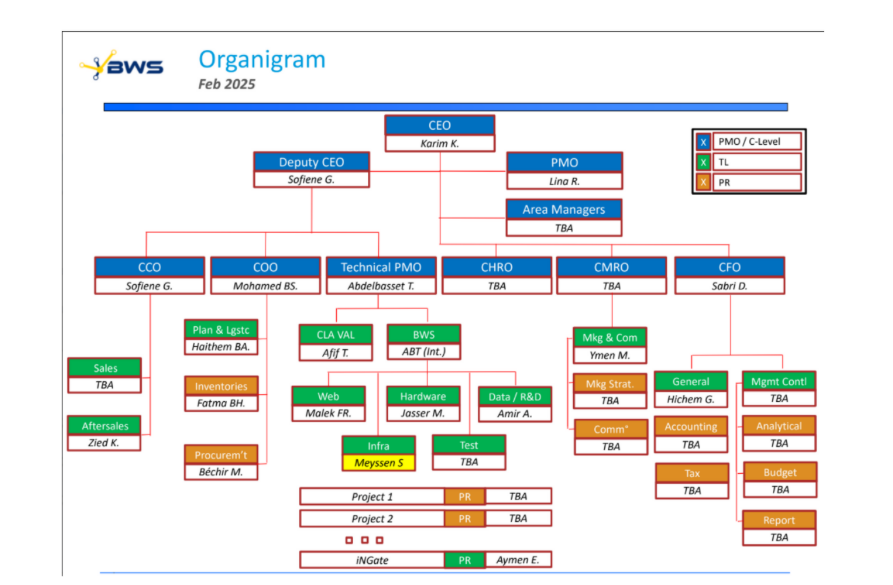
\includegraphics[width=0.75\textwidth]{Figures/organigram.png}
    \caption{Organization chart of Be Wireless Solutions}
    \label{fig:organization_chart}
\end{figure}

\subsection{Main Activities and Services}

BWS develops a wide range of industrial IoT solutions designed to improve operational efficiency, resource management, and process supervision.

\subsubsection{Energy Monitoring and Management}

BWS provides intelligent energy monitoring systems capable of collecting, analyzing, and visualizing electricity consumption data in real time. These solutions help organizations identify energy-intensive equipment, optimize consumption, reduce operational costs, and improve environmental performance.

\begin{figure}[H]
    \centering
    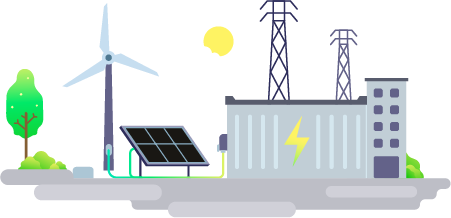
\includegraphics[width=0.7\textwidth]{Figures/electricity.png}
    \caption{Electricity consumption monitoring solution}
\end{figure}

\subsubsection{Water Monitoring Solutions}

The company offers smart water management solutions that enable remote meter reading, leak detection, abnormal consumption monitoring, and resource optimization.

\begin{figure}[H]
    \centering
    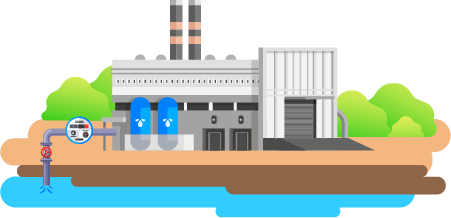
\includegraphics[width=0.7\textwidth]{Figures/water.png}
    \caption{Water consumption monitoring solution}
\end{figure}

\subsubsection{Fleet and Fuel Management}

BWS develops fleet management systems that provide real-time vehicle tracking, fuel consumption analysis, route optimization, and driver behavior monitoring.

\begin{figure}[H]
    \centering
    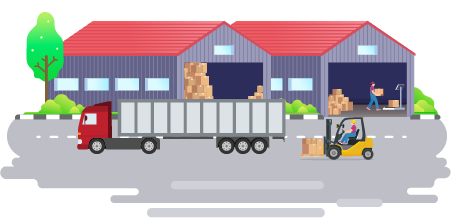
\includegraphics[width=0.7\textwidth]{Figures/fleet.png}
    \caption{Fleet and fuel management solution}
\end{figure}

\subsubsection{Remote Monitoring and Equipment Control}

The company provides remote supervision solutions that allow operators to monitor industrial equipment, detect anomalies, generate alerts, and perform remote control operations through dedicated software platforms.

\begin{figure}[H]
    \centering
    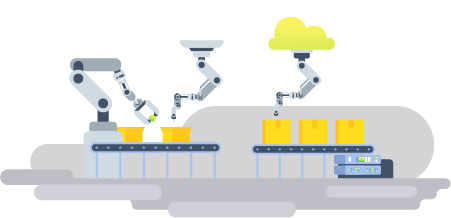
\includegraphics[width=0.7\textwidth]{Figures/equipment.png}
    \caption{Remote equipment monitoring and control}
\end{figure}

\subsubsection{Cold Chain Monitoring}

BWS also offers cold-chain monitoring systems intended for warehouses, refrigerated transportation, and pharmaceutical storage facilities. These solutions ensure compliance with temperature requirements and provide instant alerts when abnormal conditions occur.

\begin{figure}[H]
    \centering
    
\includegraphics[width=0.7\textwidth]{Figures/coldchain.png}
    \caption{Cold-chain monitoring solution}
\end{figure}

%__ Project specification
\section{Project Specification}

\subsection{Problem Statement}

Industrial IoT systems generally integrate a large number of sensors, actuators, and communication interfaces. In many cases, each new application requires dedicated firmware modifications, peripheral configuration, and hardware adaptations. This approach increases development time, reduces software reusability, and complicates system maintenance.

Moreover, industrial environments often involve heterogeneous communication protocols and interface standards. Managing these technologies through application-specific implementations creates additional complexity and limits system scalability.

To address these limitations, Be Wireless Solutions initiated the development of the IO-Box platform. The objective is to provide a configurable and reusable industrial acquisition and control system capable of simplifying peripheral integration while maintaining flexibility, portability, and maintainability.

\subsection{Presentation of the IO-Box Platform}

The IO-Box is a configurable industrial acquisition and control platform developed to facilitate the integration of sensors, actuators, and communication interfaces within industrial systems.

The platform is built around a modular embedded architecture that separates hardware-dependent components from application-level services. This approach relies on dedicated drivers, a Board Support Package (BSP), and Hardware Abstraction Layer (HAL) mechanisms to ensure portability and maintainability.

The IO-Box supports multiple categories of industrial peripherals, including analog inputs, digital inputs, digital outputs, communication interfaces, and measurement devices. Through a configurable software architecture, the platform can be adapted to different industrial use cases without significant firmware modifications.

By providing a unified interface between hardware resources and application services, the IO-Box reduces integration complexity and accelerates deployment in industrial environments.

\subsection{Project Objectives}

The main objective of this project is the design and development of the IO-Box platform capable of acquiring, processing, regulating, and transmitting industrial data in real time.

More specifically, the project aims to:

\begin{itemize}
    \item Design and implement a modular industrial acquisition and control platform.
    \item Provide a unified software abstraction layer for heterogeneous peripherals.
    \item Support configurable analog and digital input/output functionalities.
    \item Facilitate communication with external systems through industrial and IoT communication interfaces.
    \item Develop a modular software architecture based on abstraction layers and reusable software components.
    \item Ensure platform scalability for future industrial applications and system extensions.
\end{itemize}

\subsection{Development Methodology}

The development of the IO-Box platform follows the V-Model (Verification and Validation Model), a structured development methodology widely used in embedded and industrial systems.

The V-Model establishes a direct relationship between each development phase and its corresponding verification activity. This approach ensures complete traceability between system requirements, design decisions, implementation activities, and validation tests.

The descending branch of the model includes requirement analysis, system design, and software design activities. The implementation phase constitutes the central stage of the development cycle.

The ascending branch focuses on verification and validation through unit testing, integration testing, system testing, and final acceptance testing.

The adoption of the V-Model contributes to improving software quality, reducing development risks, and facilitating project management throughout the entire lifecycle.

\begin{figure}[H]
    \centering
    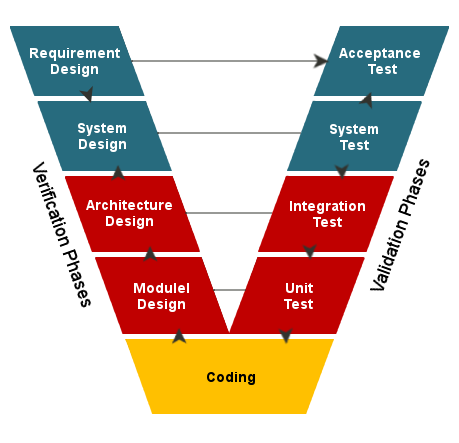
\includegraphics[width=0.75\textwidth]{Figures/v-model.png}
    \caption{V-Model development lifecycle}
    \label{fig:vmodel}
\end{figure}

\subsection{Expected Contributions}

The developed IO-Box platform is expected to significantly simplify the integration of industrial sensors and actuators while reducing deployment and maintenance efforts.

By providing a unified hardware and software architecture, the platform improves interoperability between devices and facilitates future system extensions. Furthermore, its modular design promotes software reuse and accelerates the development of new industrial applications.

The developed platform contributes to reducing development effort and deployment time by providing a standardized and reusable embedded architecture capable of supporting a wide range of industrial applications.

\section{Conclusion}

This chapter introduced the general framework of the project. The academic institution and the host company were first presented, followed by an overview of the company's activities and technological solutions. The project specifications, problem statement, objectives, and development methodology were then detailed.

The next chapter focuses on the requirements analysis and system study, providing a detailed description of the functional and technical requirements that guided the design and implementation of the IO-Box platform.
%\fancyfood[R]{\thepage}
%\renewcommand{\headrulewidth}{0.5pt}
\chapter{General Concept and System Components  }

\chaptermark{General Concept and System Components   }
\pagestyle{fancy}
\fancyhf{}
\fancyhead[HL]{Chapter 2: General Concept and System Components}
\cfoot{\thepage}

\section{Introduction}
<<<<<<< HEAD
This chapter talks about the technical setup and the main parts used to build the IO-Box platform. It covers the hardware and software that make up the system, like the STM32G474 microcontroller,  external peripherals, sensors, tools for development, and communication protocols.

The chapter also explains the main STM32 parts used in the project, such as Analog-to-Digital Converters (ADC), Digital-to-Analog Converters (DAC), timers, and Pulse Width Modulation (PWM) features.
Knowing about these technologies is important for understanding the design and how things work, which will be explained in the next chapters.
=======
This chapter presents the technical environment and the main components used in the development of the IOBOX platform. It introduces the hardware and software resources that form the basis of the system, including the STM32G474 microcontroller, external peripherals, sensors, development tools, and communication protocols.
>>>>>>> a15e0a982f2f6d5766b8147a7f12c9c22426e956


<<<<<<< HEAD
\section{General Concept of the IO-Box Platform}
The IO-Box is a customizable industrial Input/Output system that helps connect sensors, actuators, and communication tools in IoT and automation setups.
=======
\section{General Concept of the IOBOX Platform}
The IOBOX is a configurable industrial Input/Output platform designed to facilitate the integration of sensors, actuators, and industrial communication interfaces within IoT and automation systems.
>>>>>>> a15e0a982f2f6d5766b8147a7f12c9c22426e956

It works as a bridge between field devices and control systems by gathering data from sensors, handling that data, managing external equipment, and sharing information using different communication protocols.

<<<<<<< HEAD
=======
Its modular architecture allows different hardware modules and software functionalities to be integrated according to application requirements. This flexibility makes the IOBOX suitable for a wide range of industrial monitoring, automation, and data acquisition applications.
>>>>>>> a15e0a982f2f6d5766b8147a7f12c9c22426e956

The system is built with a modular design, meaning it can include various hardware parts and software features based on what's needed for each project.
This adaptability makes it useful for many industrial tasks like monitoring, automating, and collecting data.

All these features—like strong embedded processing, multiple communication options, the ability to read both analog and digital signals, and reliable storage—are combined into one easy-to-use device.
%__Part 2 of Chapter 2: General concept and system components
\section{IOBOX Hardware architecture}
The microcontroller operates from a 3.3~V power supply and can be programmed and debugged through dedicated JTAG/SWD and UART interfaces. It provides several input and output resources, including four analog input channels connected to the ADC peripherals, seven digital input channels, seven digital output channels, and four PWM outputs for actuator control applications.

For analog signal generation, the platform integrates DAC outputs capable of producing industrial-standard 4--20~mA current signals. These outputs enable the IOBOX to interface directly with industrial control equipment and monitoring systems.

The platform supports a wide range of communication protocols to ensure compatibility with industrial and IoT environments. A USB interface is available for configuration and data exchange, while an SPI interface provides high-speed communication. Multiple I\textsuperscript{2}C buses are used for sensor integration and peripheral expansion.

Industrial communication capabilities are implemented through dedicated \linebreak transceivers. To ensure compatibility with modern industrial networks, the IOBOX integrates a TCAN330GD transceiver that enables CAN FD communication between the STM32G474 and external equipment. LIN communication is achieved through the TJA1020 LIN transceiver, while RS485 communication is implemented using the THVD1410 transceiver, enabling reliable long-distance communication and Modbus RTU integration.

To extend the number of available communication channels, the architecture incorporates a TCP9548A I\textsuperscript{2}C multiplexer, which expands a single I\textsuperscript{2}C bus into eight independent channels. Additionally, a PCF8574 I/O expander controls two CD74HC4051 multiplexers, allowing the selection of up to eight UART communication channels through a reduced number of microcontroller pins.

All interfaces are routed to dedicated external connectors, facilitating the connection of sensors, actuators, and external industrial equipment. This modular and scalable architecture provides the flexibility required for industrial automation, monitoring, data acquisition, and IoT applications while maintaining the possibility of future hardware and software extensions.

Figure~\ref{fig:synoptic_architecture} presents the overall synoptic architecture of the IOBOX platform. The system is centered around the STM32G474MBTx microcontroller, which acts as the main processing unit and coordinates data acquisition, signal processing, communication, and control functions.
\begin{figure}[H]
    \centering
    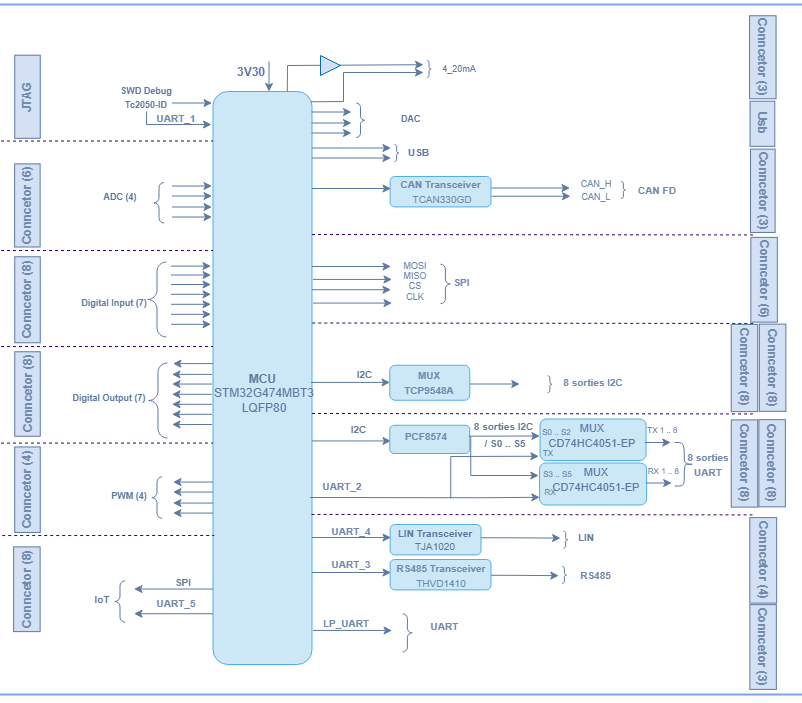
\includegraphics[width=\textwidth]{Figures/schema_synoptique.png}
    \caption{Synoptic architecture of the IOBOX platform}
    \label{fig:synoptic_architecture}
\end{figure}

\section{Hardware components}

\subsection{STM32G474MBTx Microcontroller}
At the center of the IO-Box hardware design is the STM32G474 microcontroller, a powerful chip made by STMicroelectronics. It uses the ARM Cortex-M4 processor with a floating-point unit, which makes it very good option for handling real-time signal processing and control tasks.
\begin{figure}[H]
    \centering
    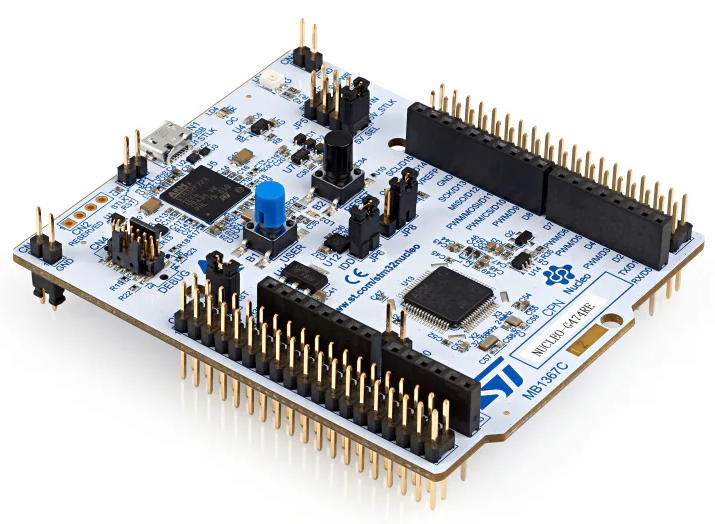
\includegraphics[width=0.55\textwidth]{Figures/nucleo-g474re.png}
    \caption{STM32G474 Microcontroller (physical package)}
    \label{fig:stm32_chip}
\end{figure}

The STM32G474 was chosen instead of the STM32F4 series because it has more ADC units (five compared to two on the F4), includes a built-in FDCAN feature, and uses a newer HAL environment. When compared to the STM32L4 series, the G474 has a faster clock speed (170 MHz versus 80 MHz) and a better analog front end, which are important for handling real-time signal processing at the needed sampling rates.

\begin{table}[H]
    \centering
    \caption{Product Attributes — STM32G474 Microcontroller}
    \label{tab:stm32g474_attributes}
    \begin{tabular}{|l|l|}
        \hline
        \textbf{Category} & Integrated Circuits, Embedded Systems, Microcontrollers \\
        \hline
        \textbf{Manufacturer} & STMicroelectronics \\
        \hline
        \textbf{Series} & STM32G4 \\
        \hline
        \textbf{Processor Core} & ARM Cortex‑M4F \\
        \hline
        \textbf{Core Size} & 32‑Bit \\
        \hline
        \textbf{Speed} & 170 MHz \\
        \hline
        \textbf{Number of I/O} & 52 \\
        \hline
        \textbf{Program Memory Size} & 512 KB Flash \\
        \hline
        \textbf{RAM Size} & 128 KB \\
        \hline
        \textbf{Data Converters} & ADC: 26 × 12‑bit; DAC: 7 × 12‑bit \\
        \hline
        \textbf{Supply Voltage} & 1.71 V – 3.6 V \\
        \hline
        \textbf{Oscillator Type} & Internal \\
        \hline
        \textbf{Operating Temperature} & –40 °C to +125 °C \\
        \hline
        \textbf{Mounting Type} & Surface Mount \\
        \hline
        \textbf{Package} & 64‑LQFP (10 × 10 mm) \\
        \hline
        \textbf{Base Product Number} & STM32G474 \\
        \hline
    \end{tabular}
\end{table}

<<<<<<< HEAD
Inside the IO-Box, the STM32G474 serves as the main processor. It handles tasks like collecting signals, processing data locally, and controlling actuators. Additionally, it manages communication with other systems using various industrial protocols, which is essential for achieving the project's goals.

\subsection{EEPROM Memory: M95M01-RDW6TP}

To manage the work with the STM32 microcontroller and make sure data is stored reliably, the IO-Box uses an external EEPROM memory called the M95M01-RDW6TP from STMicroelectronics. This device stores important information like settings, calibration data, and system logs, so the system can keep this data even when the power is turned off.
=======
Within the IOBOX, the STM32G474 acts as the central processing unit, coordinating
signal acquisition, local data processing, and actuator control. It also supervises
communication with external systems through multiple industrial protocols, making it a
key enabler of the project’s objectives.

\subsection{EEPROM Memory: M95M01-RDW6TP}

To complement the STM32 microcontroller and ensure reliable data storage, the IOBOX integrates an external EEPROM memory, specifically the M95M01‑RDW6TP from STMicroelectronics. This device provides non‑volatile storage for configuration parameters, calibration data, and system logs, allowing the platform to retain critical information even after power cycles.
>>>>>>> a15e0a982f2f6d5766b8147a7f12c9c22426e956

The M95M01-RDW6TP is a 1-Mbit serial EEPROM that is organized into 131,072 memory locations, each holding 8 bits.
It has a fast response time of 25 nanoseconds and connects through the SPI bus, which makes it easy to use with the STM32G474. It comes in an 8-pin SOIC package, making it a small and efficient option for embedded systems. It can handle up to one million write operations and keeps data safely for up to 40 years, making it a dependable choice for industrial uses where reliability is key.

\begin{table}[H]
    \centering
    \caption{Key Characteristics of M95M01‑RDW6TP EEPROM}
    \label{tab:eeprom}
    \begin{tabular}{|l|l|}
        \hline
        \textbf{Feature} & \textbf{Specification} \\
        \hline
        Manufacturer & STMicroelectronics \\
        \hline
        Type & Serial EEPROM \\
        \hline
        Capacity & 1 Mbit (131,072 × 8 bits) \\
        \hline
        Interface & SPI \\
        \hline
        Access Time & 25 ns \\
        \hline
        Package & SOIC‑8 \\
        \hline
        Endurance & 1,000,000 write cycles \\
        \hline
        Data Retention & 40 years \\
        \hline
        Operating Voltage & 1.8 V – 5.5 V \\
        \hline
    \end{tabular}
\end{table}

\begin{figure}[H]
    \centering
    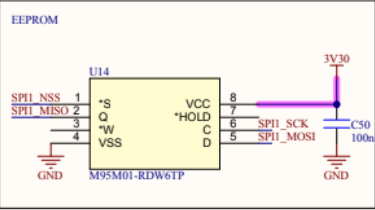
\includegraphics[width=0.5\textwidth]{Figures/eeprom.png}
    \caption{M95M01‑RDW6TP EEPROM memory chip}
    \label{fig:eeprom}
\end{figure}

\subsection{Sensors}

<<<<<<< HEAD
In the IOBox project, we added several sensors to measure different environmental and physical conditions. Our main task was to connect these sensors to the STM32G474 microcontroller, set up their settings, handle how they communicate, and do some testing to make sure the data they collect is correct. We looked closely at each sensor, learned about how they work, and wrote down their features to show how each one contributes to the whole system.
=======
In the IOBOX project, several sensors were integrated to enable environmental and physical measurements. Our work focused not only on interfacing these sensors with the STM32G474 microcontroller, but also on configuring their registers, managing communication protocols, and performing calibration to ensure accurate data acquisition. Each sensor was studied in detail, and its characteristics were documented to highlight its role within the system.
>>>>>>> a15e0a982f2f6d5766b8147a7f12c9c22426e956

\subsubsection{ENS210 Sensor}

The ENS210 is a digital sensor made by ScioSense that measures both temperature and humidity in a small size. It uses an I\textsuperscript{2}C interface to connect easily with microcontrollers like the STM32G474. The sensor is known for being accurate and using very little power, which makes it a good choice for use in systems that monitor the environment.

\begin{table}[H]
    \centering
    \caption{Key Characteristics of ENS210 Sensor}
    \label{tab:ens210}
    \begin{tabular}{|l|l|}
        \hline
        \textbf{Feature} & \textbf{Specification} \\
        \hline
        Manufacturer & ScioSense \\
        \hline
        Type & Temperature + Humidity Sensor \\
        \hline
        Interface & I\textsuperscript{2}C (16‑bit output registers) \\
        \hline
        Supply Voltage & 1.71 V – 3.6 V \\
        \hline
        Temperature Range & –40 °C to +100 °C \\
        \hline
        Temperature Accuracy & ±0.15 °C \\
        \hline
        Humidity Range & 0 – 100 \% RH \\
        \hline
       Humidity Accuracy & $\pm$2 \% RH \\
        \hline
        Package & 4‑QFN (2 × 2 mm) \\
        \hline
    \end{tabular}
\end{table}

\begin{figure}[H]
    \centering
    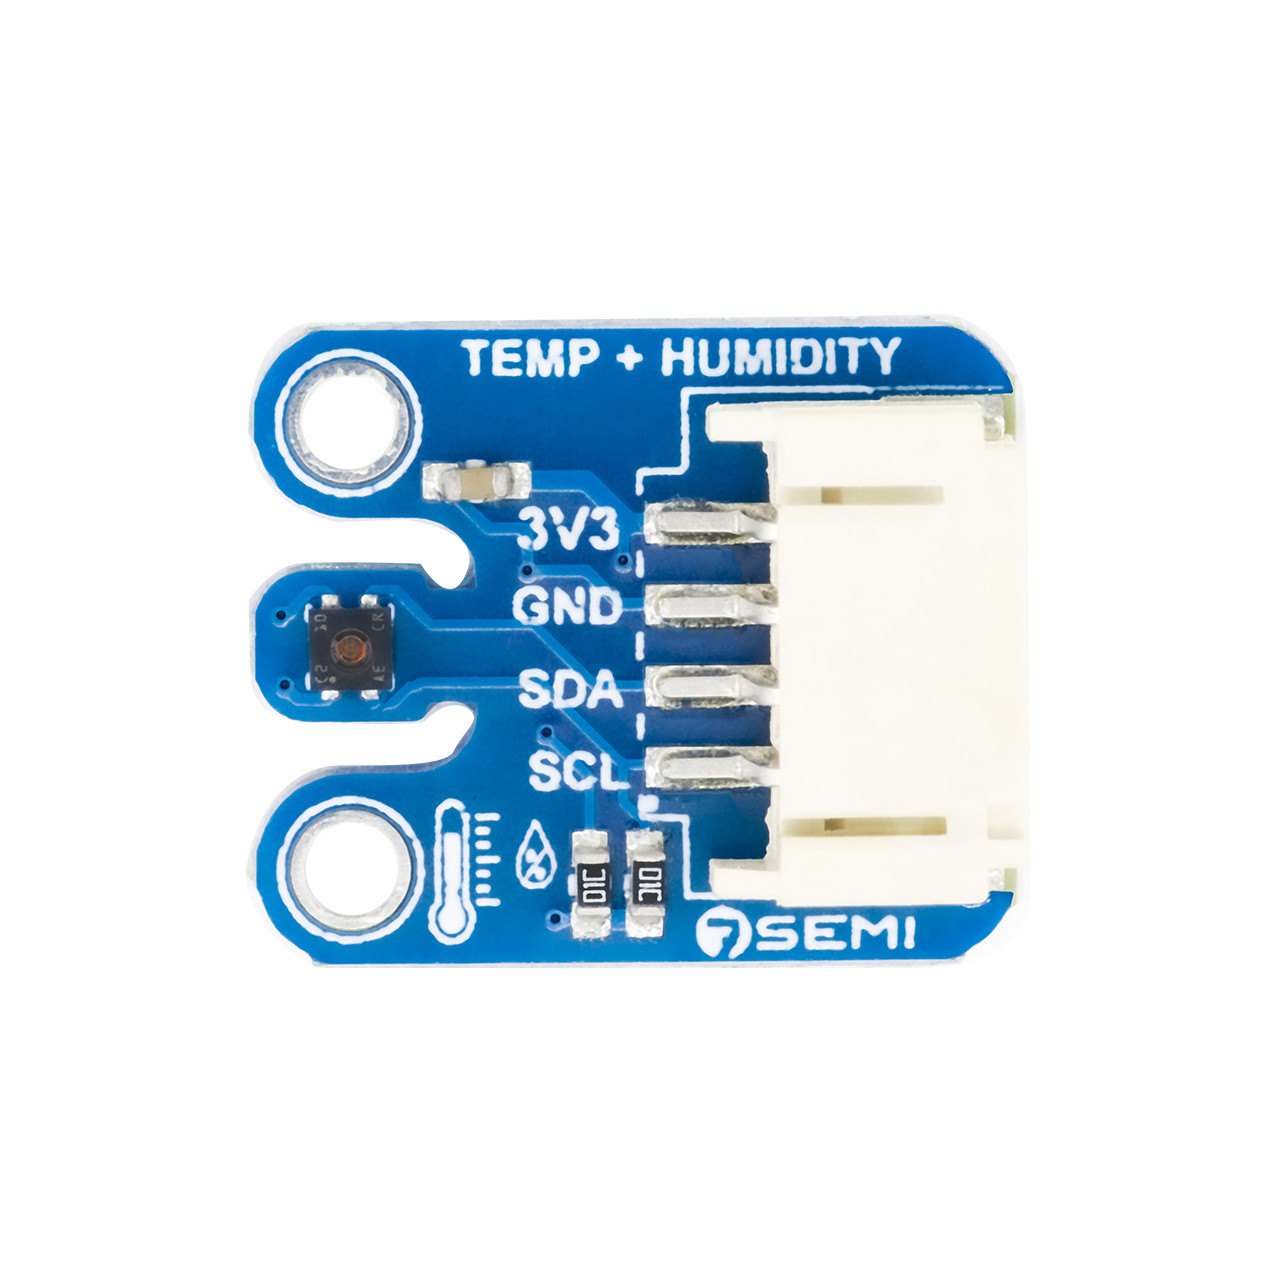
\includegraphics[width=0.3\textwidth]{Figures/ens210.jpg}
    \caption{ENS210 digital temperature and humidity sensor}
    \label{fig:ens210}
\end{figure}

\subsubsection{OPT3001DNPR Sensor}

The OPT3001DNPR is a digital light sensor made by Texas Instruments. It measures how bright the light is and shows the results in units called lux. This makes it great for uses like automatically adjusting screen brightness, controlling display backlights, and monitoring the environment. The sensor uses the I\textsuperscript{2}C communication method and has built-in calibration and a linear response over a wide range of light levels.

In the IO-Box project, the OPT3001DNPR was used to get precise light readings.
Work was done on its internal settings to set up different measurement modes, set thresholds, and run calibration processes, ensuring the sensor gave dependable data for real-time use.
\begin{table}[H]
    \centering
    \caption{Key Characteristics of OPT3001DNPR Sensor}
    \label{tab:opt3001}
    \begin{tabular}{|l|l|}
        \hline
        \textbf{Feature} & \textbf{Specification} \\
        \hline
        Manufacturer & Texas Instruments \\
        \hline
        Type & Ambient Light Sensor \\
        \hline
        Interface & I\textsuperscript{2}C \\
        \hline
        Supply Voltage & 1.6 V – 3.6 V \\
        \hline
        Measurement Range & 0.01 lux – 83,000 lux \\
        \hline
        Output Format & 16‑bit digital result in lux \\
        \hline
        Accuracy & ±10\% typical \\
        \hline
        Operating Temperature & –40 °C to +85 °C \\
        \hline
        Package & 6‑Pin WSON (2 × 2 mm) \\
        \hline
    \end{tabular}
\end{table}

\begin{figure}[H]
    \centering
    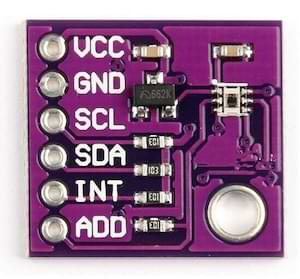
\includegraphics[width=0.3\textwidth]{Figures/opt3001.jpg}
    \caption{OPT3001DNPR ambient light sensor}
    \label{fig:opt3001}
\end{figure}

\subsubsection{HTS221TR Sensor}

The HTS221TR is a capacitive digital humidity and temperature sensor developed by STMicroelectronics. It integrates sensing elements and signal conditioning circuitry within a compact package, providing calibrated measurements through a standard I\textsuperscript{2}C interface. The sensor is designed for low-power applications while maintaining good measurement accuracy, making it suitable for environmental monitoring and industrial IoT systems.

Within the IOBOX platform, the HTS221TR is used to acquire ambient temperature and relative humidity data. Its factory-calibrated coefficients simplify integration and improve measurement reliability. Communication with the STM32G474 microcontroller is achieved through the I\textsuperscript{2}C bus, and dedicated software drivers were developed to configure the device and process sensor data.

\begin{table}[H]
    \centering
    \caption{Key Characteristics of HTS221TR Sensor}
    \label{tab:hts221}
    \begin{tabular}{|l|l|}
        \hline
        \textbf{Feature} & \textbf{Specification} \\
        \hline
        Manufacturer & STMicroelectronics \\
        \hline
        Type & Temperature + Humidity Sensor \\
        \hline
        Interface & I\textsuperscript{2}C (SPI mode not used in this project) \\
        \hline
        Supply Voltage & 1.7 V -- 3.6 V \\
        \hline
        Temperature Range & -40 °C to +120 °C \\
        \hline
        Temperature Accuracy & $\pm$0.5 °C (typ.) \\
        \hline
        Humidity Range & 0 -- 100 \% RH \\
        \hline
        Humidity Accuracy & $\pm$3.5 \% RH (typ.) \\
        \hline
        Output Resolution & 16-bit \\
        \hline
        Package & HLGA-6 (2 × 2 mm) \\
        \hline
    \end{tabular}
\end{table}

\begin{figure}[H]
    \centering
    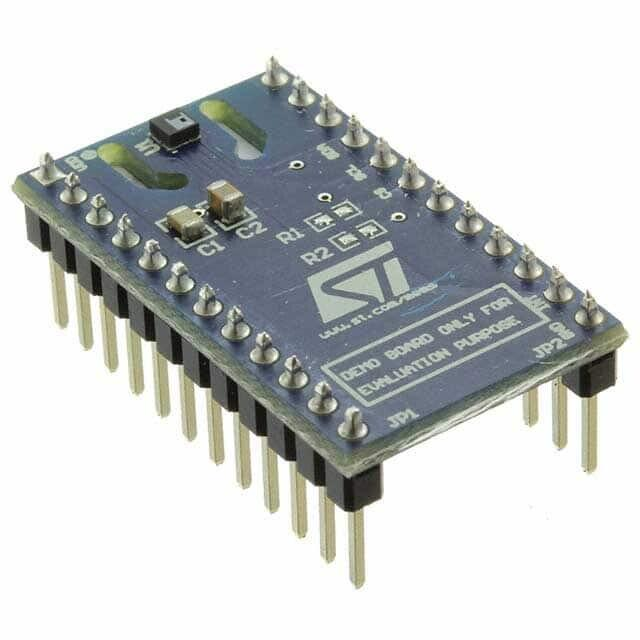
\includegraphics[width=0.3\textwidth]{Figures/hts221.jpg}
    \caption{HTS221TR temperature and humidity sensor}
    \label{fig:hts221}
\end{figure}

\section{Peripherals}

\subsection{Digital-to-Analog Converter (DAC)}
The Digital-to-Analog Converter (DAC) is an analog output peripheral integrated within the STM32G474MBTx microcontroller. It converts digital values stored in memory into continuous analog voltage levels with a resolution defined by the DAC bit width. This allows the generation of precise voltage references or analog waveforms such as sine waves, ramps, or arbitrary signals.

The DAC can operate in several modes, including software-triggered mode, timer-triggered mode, and DMA-driven mode. In timer-triggered mode, a hardware timer periodically updates the DAC output, ensuring precise and deterministic signal timing. When combined with Direct Memory Access (DMA), the DAC can continuously output precomputed waveform data without CPU intervention, significantly improving efficiency.

In the IOBox platform, the DAC is used to generate analog reference signals for actuator control. Two DAC channels are available, supporting both software-triggered and timer-triggered output modes. 

An example of DAC signal generation is illustrated in Figure~\ref{fig:dac_waveform}.

\begin{figure}[h]
\centering
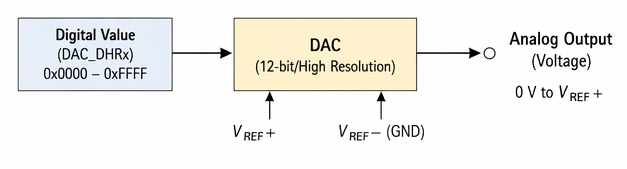
\includegraphics[width=0.65\textwidth]{Figures/dac_waveform.png}
\caption{Example of analog signal generated by DAC}
\label{fig:dac_waveform}
\end{figure}

\subsection{Analog to Digital Converter (ADC)}

The Analog‑to‑Digital Converter (ADC) is a fundamental peripheral in embedded systems, responsible for transforming continuous analog signals into discrete digital values that can be processed by the microcontroller. This conversion is essential for applications where physical phenomena such as temperature, pressure, or current must be measured and interpreted by digital logic.

In the IOBox project, ADCs are employed to acquire signals from sensors and external modules, enabling precise monitoring and control. The STM32G474 microcontroller integrates multiple high‑resolution ADC channels, allowing simultaneous sampling of different inputs. This capability is particularly important in industrial contexts where multiple signals must be captured in real time.

The operation of an ADC follows a well‑defined process. The analog input is sampled at regular intervals determined by the sampling frequency. Each sample is then quantized into a digital value according to the converter’s resolution (e.g., 12‑bit or 16‑bit). The resulting digital word represents the amplitude of the analog signal at that instant. The accuracy of this conversion depends on factors such as resolution, sampling rate, and reference voltage stability.

Key characteristics of ADCs include:
\begin{itemize}
    \item \textbf{Resolution}: Defines the number of discrete levels available.
    \item \textbf{Sampling Rate}: Determines how frequently the analog signal is measured, affecting the fidelity of dynamic signals.
    \item \textbf{Reference Voltage}: Sets the maximum measurable input range, ensuring proper scaling of the digital output.
    \item \textbf{Input Channels}: Multiple channels allow acquisition from several sensors simultaneously.
    \item \textbf{Conversion Modes}: Support for single, continuous, and DMA‑driven conversions, enabling flexible integration into firmware.
\end{itemize}

Within the IO‑Box, ADCs are used to capture sensor data such as voltage levels, current measurements, or other analog signals. These values are then processed by the firmware to generate meaningful information, trigger control actions, or communicate results to external supervisory systems.

\begin{figure}[H]
    \centering
    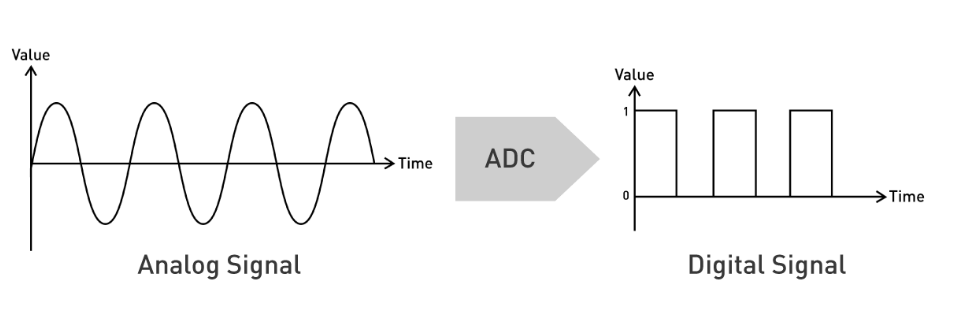
\includegraphics[width=0.70\textwidth]{Figures/ADC.png}
    \caption{Basic ADC conversion from analog input to digital output}
    \label{fig:adc}
\end{figure}

\subsection{Timers}

Timers are fundamental peripherals in the STM32G474 microcontroller, designed to provide accurate time base generation, event counting, and signal measurement. They operate by incrementing or decrementing a counter register according to a clock source, and can trigger actions when predefined values are reached.

Key functionalities of timers include:
\begin{itemize}
    \item \textbf{Time Base Generation}: Creating precise delays or periodic events.
    \item \textbf{Input Capture}: Measuring external signal characteristics such as frequency or pulse width.
    \item \textbf{Output Compare}: Generating events when the counter matches a reference value.
    \item \textbf{Synchronization}: Coordinating multiple timers for complex control tasks.
    \item \textbf{Advanced Features}: Dead‑time insertion, break inputs, and complementary outputs for safe power electronics control.
\end{itemize}

Timers are essential for scheduling tasks, measuring sensor signals, and driving peripherals that require precise timing.


\subsection{Pulse Width Modulation (PWM)}

Pulse Width Modulation (PWM) is a technique used to encode analog information into a digital waveform by varying the duty cycle of a periodic signal. In embedded systems, PWM is widely used for motor control, LED dimming, and power regulation.

PWM signals in the STM32G474 are generated using timers. The timer counts up to a predefined value stored in the auto‑reload register (ARR), while the compare register (CCR) defines the switching point of the output. The ratio between the high time and the total period represents the duty cycle. By adjusting ARR and CCR, both frequency and duty cycle can be controlled with high precision.

Key characteristics of PWM include:
\begin{itemize}
    \item \textbf{Frequency}: Determined by prescaler and ARR configuration.
    \item \textbf{Duty Cycle}: Defined by CCR relative to ARR.
    \item \textbf{Resolution}: Limited by timer bit width (typically 16‑bit).
    \item \textbf{Complementary Outputs}: Enable safe control of MOSFET drivers in half‑bridge or full‑bridge circuits.
    \item \textbf{Applications}: Motor drivers, LED dimming, switching converters, and DAC emulation.
\end{itemize}

\begin{figure}[H]
    \centering
    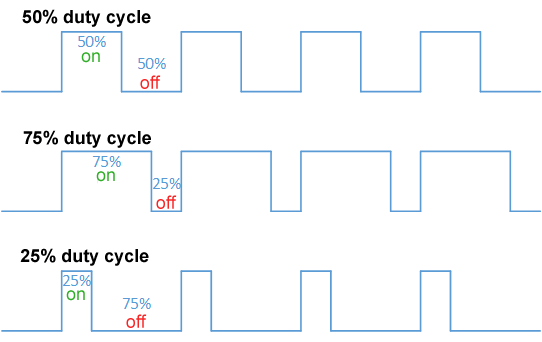
\includegraphics[width=0.6\textwidth]{Figures/Duty_Cycle_Examples.png}
    \caption{Illustration of PWM signals with different duty cycles}
    \label{fig:pwm}
\end{figure}

\section{Communication Protocols}

\subsection{I2C Protocol}
Inter-Integrated Circuit (I2C) is a synchronous, half-duplex serial communication protocol widely used for communication between integrated circuits over short distances. It relies on two bidirectional lines: the Serial Data Line (SDA) and the Serial Clock Line (SCL), both requiring pull-up resistors. The protocol follows a master-slave architecture, where the master initiates communication and generates the clock signal.

Each device connected to the bus is identified by a unique address. Data is then exchanged one byte at a time, with each byte followed by an acknowledgment bit (ACK/NACK) from the receiving device. The communication is terminated by a STOP condition. I2C supports different speed modes, including Standard Mode (100 kHz), Fast Mode (400 kHz), and higher-speed variants.

The I2C frame structure is illustrated in Figure~\ref{fig:i2c_frame}.

\begin{figure}[h]
\centering
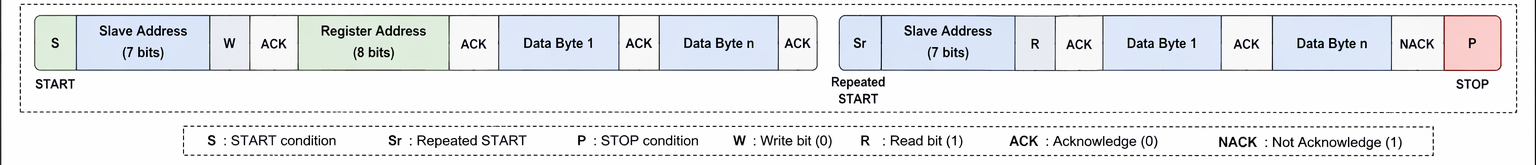
\includegraphics[width=0.7\textwidth]{Figures/i2c_frame.png}
\caption{I2C frame format}
\label{fig:i2c_frame}
\end{figure}

In this project, the I2C interface of the STM32G474MBTx is configured using the HAL library generated by STM32CubeMX. It is used to communicate with external peripherals such as sensors and low-speed devices. The implementation relies on interrupt or polling-based data transfers depending on timing constraints. Particular attention is given to bus stability, including proper pull-up resistor sizing and handling of potential communication errors such as bus busy states or missing acknowledgments.

As shown in Figure~\ref{fig:i2c_bus}, the I2C bus allows multiple slave devices.

\begin{figure}[h]
\centering
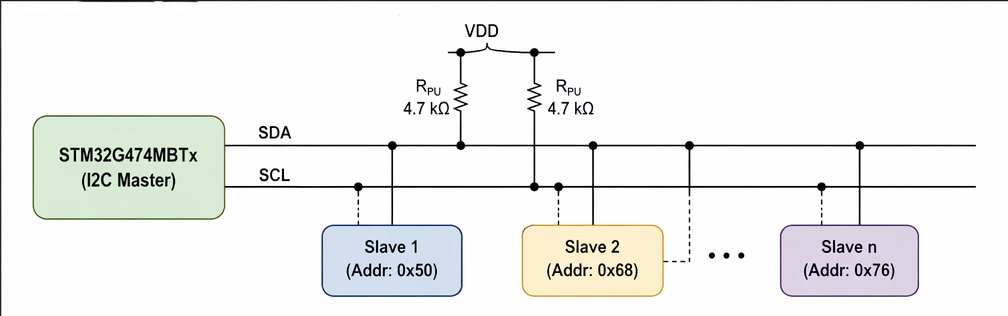
\includegraphics[width=0.7\textwidth]{Figures/i2c_bus.png}
\caption{I2C communication bus architecture}
\label{fig:i2c_bus}
\end{figure}

\subsection{Serial Peripheral Interface (SPI)}

The Serial Peripheral Interface (SPI) is a synchronous serial communication protocol widely used in embedded systems. It enables high‑speed data exchange between a microcontroller and peripheral devices such as sensors, memory modules, or communication transceivers. SPI operates in a master–slave configuration, where the microcontroller typically acts as the master, controlling the clock and data flow.

In the IOBOX project, SPI is employed to ensure reliable and efficient communication with external modules that require fast data transfer. Its simplicity and speed make it suitable for real‑time applications, particularly when multiple peripherals must be interfaced with the STM32 microcontroller.

SPI communication is based on a clock signal generated by the master device. Each bit of data is shifted out on the MOSI line while simultaneously another bit is shifted in on the MISO line. This process is synchronized by the clock (SCLK), ensuring deterministic timing. The communication sequence typically follows these steps: the master activates the Chip Select (CS) line of the desired slave, provides the clock signal, transmits data bit‑by‑bit on MOSI while receiving data on MISO, samples the data according to the configured mode, and finally deactivates the CS line to end the session. This mechanism allows full‑duplex communication, meaning data can be transmitted and received simultaneously.

SPI supports four modes of operation (Mode 0 to Mode 3), determined by the configuration of clock polarity (CPOL) and clock phase (CPHA). This flexibility ensures compatibility with a wide range of peripheral devices. Key characteristics of SPI include its high speed (operating at several MHz), simple wiring with four main signals (MOSI, MISO, SCLK, CS), and scalability through multiple slave connections.

\begin{figure}[H]
    \centering
    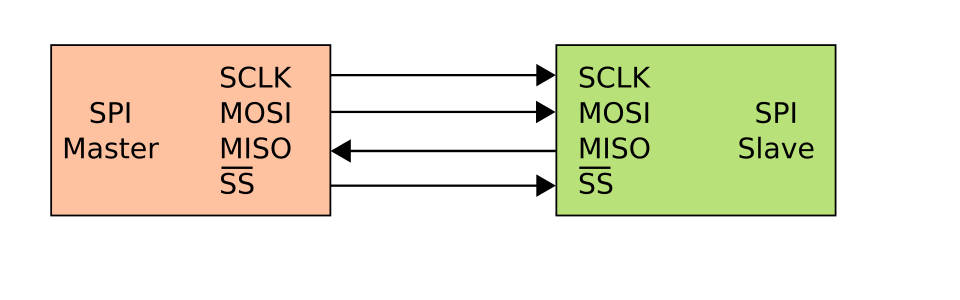
\includegraphics[width=0.65\textwidth]{Figures/spi_diagram.png}
    \caption{Basic SPI communication between master and slave devices}
    \label{fig:spi}
\end{figure}

\subsection{UART Protocol}
Universal Asynchronous Receiver-Transmitter (UART) is an asynchronous serial communication protocol that enables full-duplex data exchange between devices without a shared clock signal. Data is transmitted over two lines: Transmit (TX) and Receive (RX). Synchronization between devices is achieved by configuring identical communication parameters, including baud rate, data bits, parity, and stop bits.

Each data frame typically consists of a start bit, followed by a configurable number of data bits (usually 8), an optional parity bit for error detection, and one or more stop bits. Unlike synchronous protocols, UART does not include a clock line, making it simpler but more sensitive to timing mismatches.

In this project, UART is used for communication between the STM32 microcontroller and external systems such as a host computer or other embedded modules. It plays a key role in debugging, logging, and real-time data exchange. The implementation uses the STM32 HAL drivers with support for interrupt-driven and DMA-based transmission to ensure efficient and non-blocking communication. Error handling mechanisms, including overrun, framing, and noise errors, are also considered to improve communication reliability.

The UART frame structure is illustrated in Figure~\ref{fig:uart_frame}.

\begin{figure}[h]
\centering
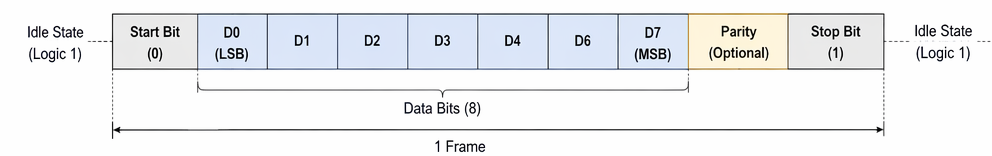
\includegraphics[width=0.9\textwidth]{Figures/uart_frame.png}
\caption{UART frame format}
\label{fig:uart_frame}
\end{figure}


\subsection{RS485 Communication}
RS485 is a robust differential serial communication standard widely used in industrial environments due to its high noise immunity and long-distance capabilities. Unlike single-ended UART communication, RS485 transmits data over a differential pair of lines (A and B), where the information is encoded as a voltage difference between the two conductors. This approach significantly reduces susceptibility to electromagnetic interference and ground potential differences.

The RS485 standard supports half-duplex communication in multi-drop configurations, allowing multiple nodes to share the same bus. However, only one device can transmit at a time, which requires proper bus arbitration at the software level or through protocol design.

In this project, RS485 serves as the physical layer for Modbus RTU communication. A dedicated UART peripheral (USART3) is used with an external RS485 transceiver to convert TTL logic levels to differential signals. Direction control is managed in software, as described in Chapter 3.

Before transmission, the microcontroller sets the DE pin high to enable the driver stage. After sending the data frame, the DE pin is reset to return the transceiver to reception mode. This timing control is critical to avoid bus contention. The communication is typically used for reliable data exchange in noisy environments, especially when longer cable lengths are required compared to standard UART.

Figure~\ref{fig:rs485_bus} illustrates a typical RS485 bus configuration.

\begin{figure}[h]
    \centering
    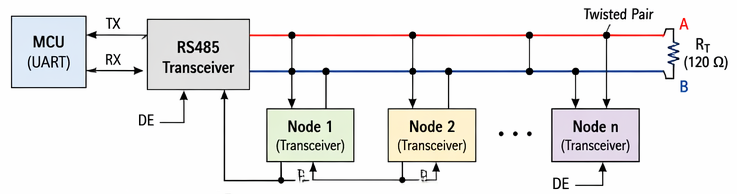
\includegraphics[width=0.65\textwidth]{Figures/rs485_bus.png}
    \caption{RS485 differential bus with multi-node configuration}
    \label{fig:rs485_bus}
\end{figure}

\subsection{Modbus Protocol}

Modbus is one of the most widely used industrial communication protocols for exchanging data between electronic devices. Originally developed by Modicon in 1979, it follows a client-server (master-slave) architecture and enables communication between programmable logic controllers (PLCs), sensors, actuators, Human-Machine Interfaces (HMIs), and embedded systems.

Modbus defines a standardized message structure that allows devices from different manufacturers to communicate using a common protocol. Two main variants are commonly used: Modbus RTU, which operates over serial communication interfaces such as RS232 and RS485, and Modbus TCP, which operates over Ethernet networks.

In the IOBOX project, Modbus RTU is implemented over the RS485 physical layer to ensure reliable communication in industrial environments. The STM32G474 microcontroller acts as either a Modbus master or slave depending on the application requirements. Through Modbus registers, external systems can access sensor measurements, configuration parameters, status information, and control commands.

In this project, the IOBox operates as a Modbus RTU slave at address 0x01, communicating over RS485 at 19,200 bps. The slave implementation supports function codes FC01 through FC06, FC15, and FC16. Input registers expose real-time sensor measurements (temperature, humidity, illuminance) to any connected Modbus master, and holding registers allow actuator control. The implementation details are described in Chapter 3.

A Modbus RTU frame consists of four main fields:

\begin{itemize}
    \item \textbf{Slave Address}: Identifies the target device.
    \item \textbf{Function Code}: Specifies the requested operation.
    \item \textbf{Data Field}: Contains transmitted data or register information.
    \item \textbf{CRC Field}: Provides error detection for frame integrity.
\end{itemize}

\begin{figure}[H]
    \centering
    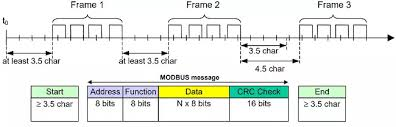
\includegraphics[width=0.8\textwidth]{Figures/modbus_rtu_frame.jpg}
    \caption{Typical Modbus RTU frame structure}
    \label{fig:modbus_frame}
\end{figure}

To ensure compatibility with standard industrial devices, the implementation supports a subset of Modbus function codes, classified according to their role in data access and control:

\begin{table}[H]
    \centering
    \caption{Supported Modbus Function Codes in the IOBOX Platform}
    \label{tab:modbus_function_codes}
    \begin{tabular}{|c|c|p{7cm}|}
    \hline
    \textbf{Function Code} & \textbf{Name} & \textbf{Description} \\
    \hline
    FC01 & Read Coils & Reads digital output states (ON/OFF status) \\
    \hline
    FC02 & Read Discrete Inputs & Reads digital input signals from sensors or switches \\
    \hline
    FC03 & Read Holding Registers & Reads configuration and control registers (16-bit) \\
    \hline
    FC04 & Read Input Registers & Reads real-time measurement data (sensor values) \\
    \hline
    FC05 & Write Single Coil & Controls a single digital output (ON/OFF command) \\
    \hline
    FC06 & Write Single Register & Writes a single 16-bit configuration or control value \\
    \hline
    FC15 & Write Multiple Coils & Updates multiple digital outputs in one request \\
    \hline
    FC16 & Write Multiple Registers & Writes multiple registers for bulk configuration/control \\
    \hline
    \end{tabular}
\end{table}

This classification enables structured interaction with the IOBOX memory map, separating real-time acquisition data (input registers) from controllable parameters (holding registers). It also ensures interoperability with a wide range of Modbus-compatible supervisory systems such as SCADA platforms and PLCs.

\subsection{Controller Area Network (CAN)}

The Controller Area Network (CAN) is a robust serial communication protocol originally developed for automotive applications, but now widely used in industrial and embedded systems. It enables reliable data exchange between multiple devices without requiring a central host, making it ideal for distributed control systems.

In the IOBOX project, CAN is employed to ensure communication with industrial equipment and sensors that demand high reliability and fault tolerance. Its ability to handle multiple nodes on a single bus makes it particularly suitable for environments where numerous devices must share information in real time.

CAN communication is based on a message‑oriented protocol. Instead of addressing specific devices directly, each message carries an identifier that defines its priority and content. This allows multiple nodes to listen simultaneously and decide whether to act on the received data. The arbitration mechanism ensures that when two nodes attempt to transmit at the same time, the message with the highest priority (lowest identifier value) wins, while the other node waits until the bus is free. This guarantees deterministic communication without collisions.

Key characteristics of CAN include:
\begin{itemize}
    \item \textbf{Multi‑master capability}: Any node can initiate communication when the bus is idle.
    \item \textbf{Error detection and handling}: Built‑in mechanisms such as CRC checks, acknowledgment bits, and error frames ensure data integrity.
    \item \textbf{Priority‑based arbitration}: Messages are prioritized by identifiers, ensuring that critical data is transmitted first.
    \item \textbf{Scalability}: Supports up to 112 nodes on a single bus, making it suitable for complex systems.
    \item \textbf{Speed}: Operates up to 1 Mbps in classical CAN, and higher in CAN FD (Flexible Data‑Rate), which extends payload size and transmission speed.
\end{itemize}

\begin{figure}[H]
    \centering
    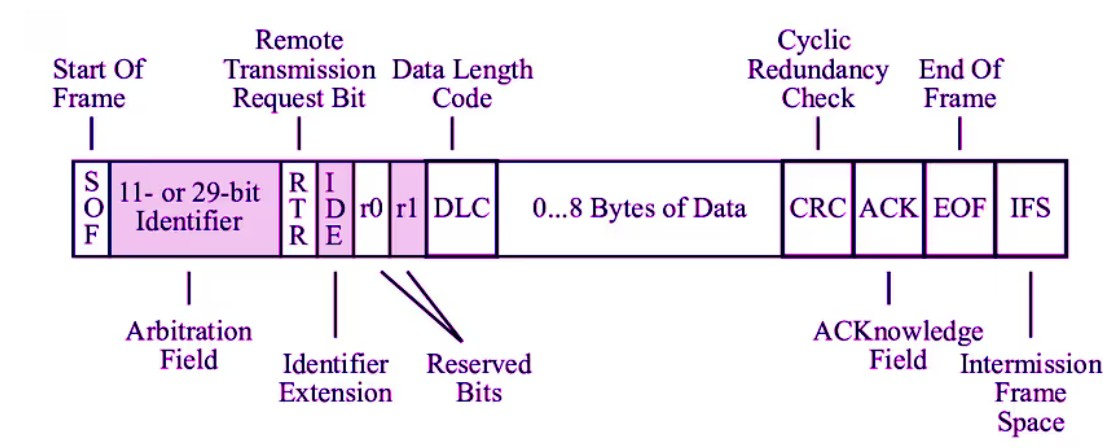
\includegraphics[width=0.70\textwidth]{Figures/trame_can.jpg}
    \caption{Basic CAN frame}
    \label{fig:can_frame}
\end{figure}

In practice, CAN uses two differential lines, CAN\_H and CAN\_L, to transmit data. This differential signaling improves noise immunity and allows reliable communication even in electrically harsh environments. Each frame consists of fields such as the start of frame, identifier, control bits, data payload, CRC, and end of frame, ensuring structured and error‑resistant communication.

\begin{figure}[H]
    \centering
    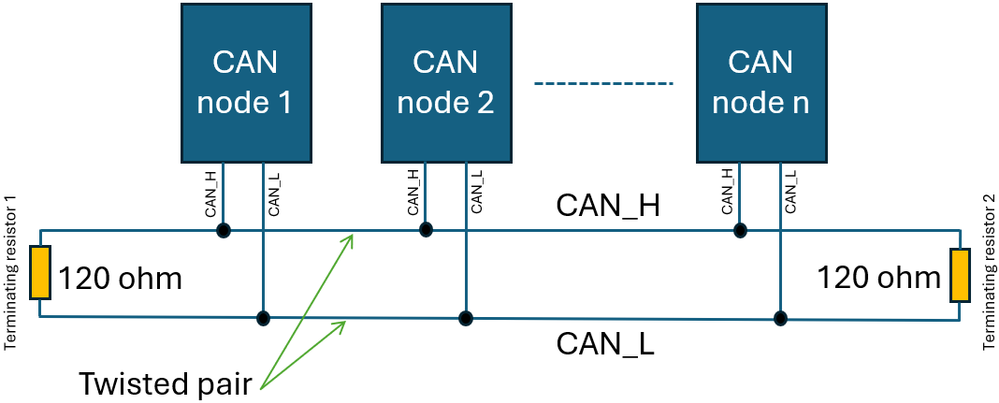
\includegraphics[width=0.70\textwidth]{Figures/can_diagram.png}
    \caption{Basic CAN bus communication with multiple nodes}
    \label{fig:can_bus}
\end{figure}

\subsection{LIN Protocol}
\nobreak{}
Local Interconnect Network (LIN) is a low-cost serial communication protocol designed for distributed control systems, particularly in automotive applications. It operates on a single-wire physical layer and follows a strict master-slave architecture where the master node controls the entire bus communication schedule.

Unlike event-driven protocols, LIN is time-triggered, meaning communication is organized into predefined frames sent at fixed intervals. Each frame consists of a header transmitted by the master and a response transmitted by a slave node. The header includes a break field (used to signal the start of a frame), a synchronization byte, and an identifier field that determines which node should respond.

The data response typically contains up to 8 bytes, followed by a checksum used for error detection. LIN achieves deterministic timing by enforcing strict scheduling, making it suitable for non-critical but predictable control tasks.

In this project, LIN communication is implemented using the STM32 UART peripheral configured in LIN mode. The hardware support simplifies break detection and synchronization field handling, reducing software complexity. The system can therefore reliably detect frame boundaries and process incoming data with minimal CPU overhead.

The LIN frame structure is shown in Figure~\ref{fig:lin_frame}.

\begin{figure}[h]
\centering
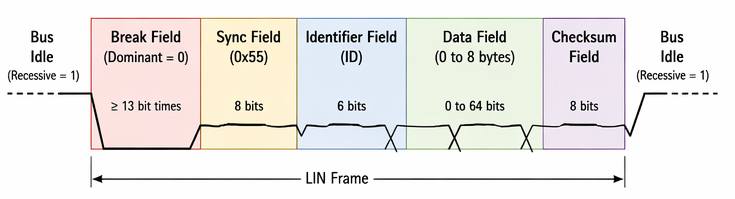
\includegraphics[width=0.8\textwidth]{Figures/lin_frame.png}
\caption{LIN frame structure}
\label{fig:lin_frame}
\end{figure}

\section{Software tools}

\subsection{Visual Studio Code}
Visual Studio Code (VS Code) is a lightweight yet powerful source code editor optimized for modern software development. It supports multiple programming languages and provides advanced features such as syntax highlighting, intelligent code completion, and debugging tools. 

In this project, Visual Studio Code was used as the primary text editor for documentation, script editing, and Git-based version control. Extensions such as Git Graph enabled visualization of commit history, branch management, and tracking of code evolution across the development team.

\begin{figure}[H]
    \centering
    
\includegraphics[width=0.2\textwidth]{Figures/vs_code.jpeg}
    \caption{Visual Studio Code interface}
    \label{fig:vscode}
\end{figure}

\subsection{IAR Embedded Workbench}
IAR Embedded Workbench (IAR EW) is a professional integrated development environment (IDE) dedicated to embedded systems programming, particularly for microcontrollers such as the STM32 family. It provides a highly optimized C/C++ compiler, advanced debugging capabilities, and efficient project management tools. 

In this project, IAR EW was used for firmware development, compilation, and debugging. Its powerful optimization features contributed to generating efficient and reliable embedded code, which is critical for real-time applications and resource-constrained systems\cite{21}.

\begin{figure}[H]
    \centering
    
\includegraphics[width=0.2\textwidth]{Figures/iar_workbench.png}
    \caption{IAR Embedded Workbench IDE}
    \label{fig:iar}
\end{figure}

\subsection{STM32CubeMX}
STM32CubeMX is a graphical configuration tool developed by STMicroelectronics for STM32 microcontrollers. It allows developers to easily configure peripherals, clock settings, and pin assignments through an intuitive interface. The tool also generates initialization code based on the selected configuration, significantly reducing development time and minimizing configuration errors. 

In this project, STM32CubeMX was used in a limited capacity: it was invoked once at the beginning of the project to generate the initial project skeleton, configure the system clock (HSI PLL at 170 MHz), and enable the Serial Wire Debug interface. The peripheral initialization functions that CubeMX would normally generate were intentionally not used. Instead, all peripheral drivers were developed as handwritten BSP (Board Support Package) modules, which are described in detail in Chapter 3. CubeMX thus served exclusively as a project scaffolding and clock configuration tool.

\begin{figure}[H]
    \centering
    
\includegraphics[width=0.4\textwidth]{Figures/stm32cubemx.png}
    \caption{STM32CubeMX configuration interface}
    \label{fig:cubemx}
\end{figure}

\subsection{GitLab}

GitLab was used as the version control and collaboration platform throughout the project. The repository was organized by module (BSP, Managers, Application), with branches used to isolate feature development and avoid conflicts during parallel work. Commit history served as a development log, and merge requests were used to review code before integrating changes into the main branch.

\begin{figure}[H]
    \centering
    
\includegraphics[width=0.2\textwidth]{Figures/gitlab_logo.png}
    \caption{GitLab logo}
    \label{fig:gitlab}
\end{figure}

\subsection{Conclusion}

In this chapter, we presented the general concept and system components of the IO‑Box project. We began with the synoptic diagram, which outlined the main functional phases of acquisition, filtering, regulation, and transmission/actuation. We then introduced the software architecture, organized into four distinct layers (HAL, BSP, Manager, and Application), and complemented this with the hardware architecture, highlighting the STM32G474 microcontroller, power supply design, communication interfaces, and peripheral modules. Finally, we described the development tools and protocols that support the implementation of the system.

By establishing this technical foundation, Chapter 3 has clarified the resources and methodologies that will be employed in the realization phase. The next chapter will be dedicated to the practical implementation of the IO‑Box, detailing the firmware design, register configuration, BSP development, and integration of sensors and actuators into a coherent and functional platform.
%\fancyfood[R]{\thepage}
%\renewcommand{\headrulewidth}{0.5pt}
\chapter{Design and Practical Implementation}

\chaptermark{Design and Practical Implementation}
\pagestyle{fancy}
\fancyhf{}
\fancyhead[HL]{Chapter 3: Design and Practical Implementation}
\cfoot{\thepage}

\section{Introduction}
The preceding chapters established the project context, defined the platform requirements, 
and presented the hardware components and communication protocols that form the technical 
foundation of the IOBOX platform. This chapter details the design decisions and practical 
implementation work carried out to bring that foundation into a functional embedded system.

The implementation is organized around a layered software architecture that separates 
hardware-specific code from higher-level application logic. At the lowest level, a Board 
Support Package (BSP) provides direct peripheral drivers for every hardware interface 
present on the platform. Above it, a Manager layer encapsulates the communication 
protocols and sensor drivers, exposing clean, hardware-independent APIs to the rest of 
the system. At the top, the Application layer coordinates all modules through a 
lightweight cooperative task scheduler and assembles sensor data into structured 
output frames.

The chapter begins by describing the hardware architecture of the IOBOX platform, 
followed by a detailed account of the software architecture and its constituent layers. 
Each subsection covers the design rationale, the implementation approach, and the key 
technical choices made during development. The chapter concludes with a summary of the 
results obtained and a discussion of the platform's readiness for industrial deployment.
\section{Hardware architecture}


\section{Software Architecture}

The firmware of the IOBOX platform is organised into three distinct horizontal layers: 
the Board Support Package (BSP), the Manager layer, and the Application layer. This 
separation was adopted to isolate hardware-specific code from protocol logic and 
application behaviour, enabling each layer to evolve independently. A central 
configuration file, \texttt{feature\_config.h}, governs the compile-time inclusion of 
every hardware feature through preprocessor flags, ensuring that only the peripherals 
and protocols required for a given deployment are compiled into the firmware binary.

A single global structure, \texttt{SystemBoard}, declared in 
\texttt{feature\_config.h} and instantiated in \texttt{main.c}, serves as the shared 
data exchange point between all layers. It aggregates real-time sensor readings, CAN 
frame data, and status information, and is accessed directly by the Manager and 
Application layers during each execution cycle.

% --- Figure: layered software architecture diagram ---
\begin{figure}[H]
    \centering
    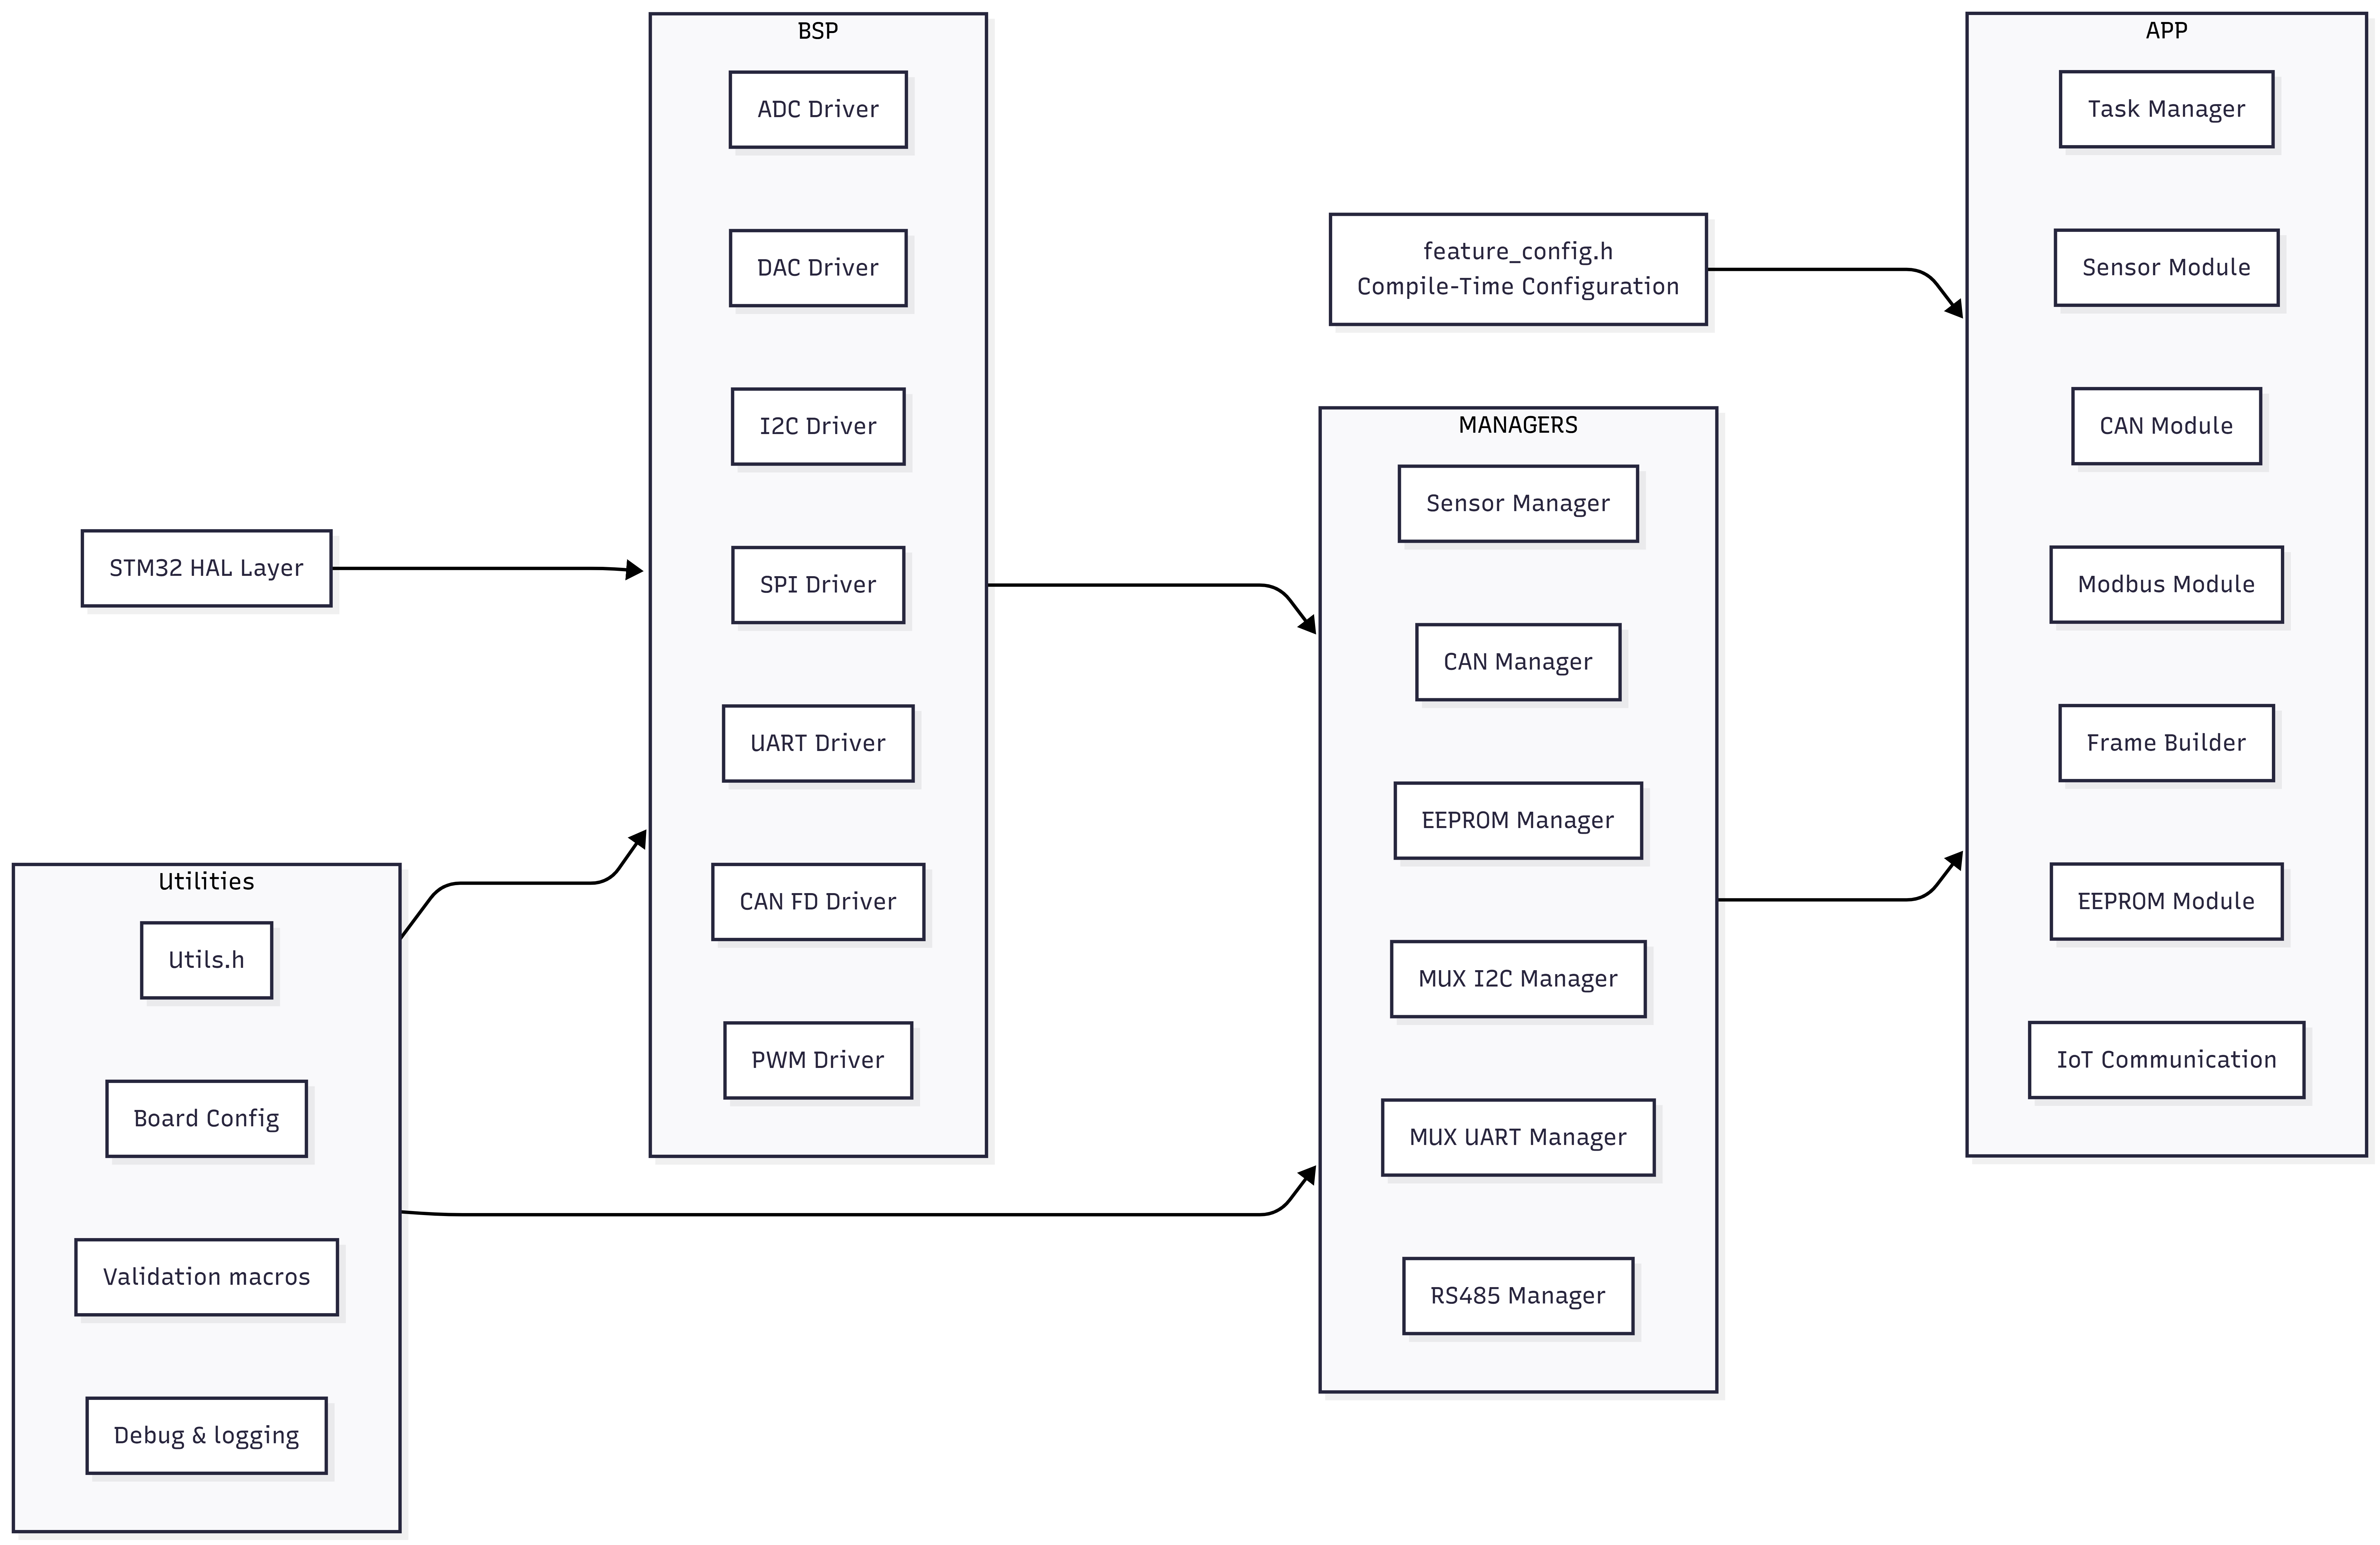
\includegraphics[width=0.75\textwidth]{Figures/software_architecture.png}
    \caption{Layered software architecture of the IOBOX platform}
    \label{fig:software_architecture}
\end{figure}

The following subsections describe each layer in detail, from the lowest hardware 
abstraction level up to the application logic.

%------------------------------------------------------------------
\subsection{Board Support Package Layer}
%------------------------------------------------------------------

The Board Support Package constitutes the lowest layer of the firmware stack. It 
provides a collection of peripheral driver modules, each encapsulating the 
initialisation, configuration, and data transfer routines for a single hardware 
interface. By confining all register-level and HAL-level operations to this layer, the 
upper layers are shielded from hardware-specific details and can interact with 
peripherals exclusively through the BSP's public API.

Each BSP module follows a consistent structure: a header file located under 
\texttt{BSP/Inc/} declares the public API, while the corresponding source file under 
\texttt{BSP/Src/} contains the implementation. The platform exposes BSP modules for the 
following peripheral categories.

Serial communication interfaces are covered by \texttt{BSP\_USART1}, 
\texttt{BSP\_USART2}, \texttt{BSP\_UART5}, and \texttt{BSP\_LPUART1} for general-purpose 
asynchronous communication, by \texttt{BSP\_RS485} for the half-duplex differential bus 
used by the Modbus RTU stack, by \texttt{BSP\_LIN} for the single-wire LIN bus, and by 
\texttt{BSP\_UART\_MUX} for the software-controlled UART channel multiplexer. 
High-speed synchronous communication is handled by three independent SPI drivers: 
\texttt{BSP\_SPI1}, \texttt{BSP\_SPI2}, and \texttt{BSP\_SPI4}. Sensor and 
peripheral expansion buses are served by \texttt{BSP\_I2C2} and \texttt{BSP\_I2C3}, 
complemented by \texttt{BSP\_I2C\_MUX}, which controls the TCA9548A eight-channel I\textsuperscript{2}C 
multiplexer. The CAN interface is abstracted by \texttt{CAN1\_BSP}, and digital 
input/output operations are centralised in \texttt{BSP\_DigitalIO}.

Analog peripherals are equally covered: four ADC drivers (\texttt{ADC1\_BSP}, 
\texttt{ADC3\_BSP}, \texttt{ADC4\_BSP}, \texttt{ADC5\_BSP}) expose acquisition 
functions for each active conversion channel, while two DAC drivers 
(\texttt{BSP\_DAC1} and \texttt{BSP\_DAC2}) provide voltage output generation. 
Four timer drivers (\texttt{TIM1\_BSP} through \texttt{TIM4\_BSP}) manage 
time-base and PWM generation. A low-power management module, \texttt{BSP\_LowPower}, 
groups the power mode transition routines.

This modular decomposition means that porting the firmware to a different STM32 
variant requires changes only within the BSP layer, leaving the Manager and 
Application layers unmodified.

%------------------------------------------------------------------
\subsection{Manager Layer}
%------------------------------------------------------------------
Three sensor manager modules were developed, one per physical sensor, each
handling I\textsuperscript{2}C multiplexer channel selection, register-level communication, and
raw-to-physical conversion.

The HTS221TR manager drives the STMicroelectronics capacitive humidity and
temperature sensor connected to I\textsuperscript{2}C multiplexer channel 0.  Subsequent acquisitions apply linear interpolation between
these reference points to convert the 16-bit raw ADC output into calibrated
temperature in degrees Celsius and relative humidity in percent, as shown in
Equations~\ref{eq:hts_rh} and~\ref{eq:hts_temp}.

\begin{equation}
\label{eq:hts_rh}
\%\mathrm{RH} = H_{0,\mathrm{rH}} +
\frac{(H_{1,\mathrm{rH}} - H_{0,\mathrm{rH}}) \cdot (\mathrm{raw} - H_{0,T_{0}})}
     {H_{1,T_{0}} - H_{0,T_{0}}}
\end{equation}

\begin{equation}
\label{eq:hts_temp}
T\,[^\circ\mathrm{C}] = T_{0,\mathrm{degC}} +
\frac{(T_{1,\mathrm{degC}} - T_{0,\mathrm{degC}}) \cdot (\mathrm{raw} - T_{0,\mathrm{out}})}
     {T_{1,\mathrm{out}} - T_{0,\mathrm{out}}}
\end{equation}

Data readiness is verified by polling the sensor's status register before each
acquisition. If the data-ready flag is not asserted within a configurable retry
count, the acquisition routine returns a timeout status without blocking the
system further.

The ENS210 manager interfaces with the ScioSense combined temperature and
humidity sensor on multiplexer channel~2. The module operates in single-shot
mode: a measurement is triggered by writing to the sensor's start register, a
fixed 10-millisecond settling delay is applied, and the 16-bit raw temperature
and humidity registers are then read. Conversion follows the datasheet-specified
formulae: temperature is obtained as $T_K = \mathrm{raw}/64$, then converted to
Celsius by subtracting 273.15; relative humidity is obtained as
$\%\mathrm{RH} = \mathrm{raw}/512$.

The OPT3001DNPR manager drives the Texas Instruments ambient light sensor on
multiplexer channel~1. The sensor is configured at initialisation by writing a
control word to its configuration register, selecting continuous conversion mode,
automatic full-scale range, and an 800-millisecond conversion time. The 16-bit
result register encodes the measurement as a four-bit binary exponent and a
twelve-bit mantissa; the illuminance in lux is recovered by the expression
$E_{\mathrm{lux}} = \mathrm{mantissa} \times 0.01 \times 2^{\mathrm{exponent}}$.

In all three managers, the I\textsuperscript{2}C multiplexer channel is selected at the start of
each transaction and disabled upon completion, preventing bus contention between
sensors sharing the same physical I\textsuperscript{2}C bus.

\subsubsection{Modbus RTU Manager}

The Modbus RTU stack provides both master and slave roles over the RS485 physical
layer and is entirely self-contained within a single manager module. 
The slave role, which is active in the current platform configuration, operates through
interrupt-driven reception. Eight function codes are supported: FC01, FC02, FC03,
FC04, FC05, FC06, FC15, and FC16. Frames addressed to other slaves are silently
discarded; frames with invalid CRC are dropped without response, as required by the
Modbus RTU specification. Following each handled frame, the receiver is re-armed
immediately to avoid missing subsequent requests.

\subsubsection{CAN Manager}

CAN frame reception is managed by a dedicated module that decouples the 
asynchronous nature of CAN bus traffic from the periodic execution rhythm of 
the Application layer. Because CAN frames can arrive at any time, independently 
of the firmware's scheduling cycle, the manager introduces an intermediate 
buffering stage between the BSP reception interface and the rest of the system. 
Incoming frames are captured and held as they arrive; the Application layer then 
retrieves and consumes them at its own cadence without any risk of frame loss 
during burst traffic conditions. Once processed, the received data is written 
into the CAN-related fields of the shared \texttt{SystemBoard} structure, making 
it immediately available to any other module that consults the platform's central 
data store.
\subsubsection{EEPROM Manager}

Non-volatile data persistence is managed by \texttt{EEPROM\_manager.c}, which 
interfaces with the M95M01-RDW6TP serial EEPROM via the SPI BSP layer. The 
manager exposes store and load primitives consumed by the Application layer to 
persist the \texttt{DataFrame} structure across power cycles.

\subsection{Filter Manager}

Industrial sensor signals are rarely clean: electrical interference, thermal 
gradients, and inherent sensor noise introduce unwanted fluctuations into raw 
measurements that, if left unprocessed, degrade the accuracy of the data 
delivered to the application layer. To address this requirement without coupling 
noise-reduction logic to individual sensor drivers, the IOBOX firmware provides a 
dedicated, generic signal processing module implemented in 
\texttt{Filter\_Manager.c} and \texttt{Filter\_Manager.h}.



The six filter algorithms provided by the module are described individually below.

%------------------------------------------------------------------
\subsubsection{Exponential Moving Average Filter}
%------------------------------------------------------------------

\paragraph{Purpose.}
The Exponential Moving Average (EMA) is a low-pass filter designed to smooth 
noisy sensor readings by weighting recent samples more heavily than older ones 
while discarding neither.

\paragraph{Principle.}
Each output value is a weighted combination of the current raw input and the 
previous filtered output. The weight assigned to the new sample is controlled 
by a single configurable parameter, so the filter can be made to respond quickly 
to real signal changes or to suppress short-lived noise spikes, depending on the 
application.

\paragraph{Main Equation.}
\begin{equation}
    y[n] = \alpha \cdot x[n] + (1 - \alpha) \cdot y[n-1]
    \label{eq:ema}
\end{equation}

\paragraph{Parameters.}
$x[n]$ is the current raw sample, $y[n-1]$ is the previous filtered output 
stored in \texttt{prev\_output}, and $\alpha \in (0,\,1]$ is the smoothing 
factor: values near zero produce heavy smoothing with slow response, while values 
near one allow fast tracking with minimal noise reduction.


\paragraph{Advantages.}
The EMA requires only two floating-point multiplications and one addition per 
update step, making it the least computationally demanding filter in the library. 
Its constant memory footprint and the absence of a ring buffer make it directly 
suitable for resource-constrained microcontrollers. The single parameter 
\texttt{alpha} provides a simple and intuitive tuning knob.

\paragraph{Disadvantages.}
Because all past samples influence the output with exponentially decaying weights, 
the EMA has no finite settling time after a large step change in the input: the 
output approaches the new level asymptotically. Additionally, the degree of 
smoothing depends implicitly on the sampling rate; if the rate changes, the 
effective cutoff behaviour changes as well unless \texttt{alpha} is retuned.

\paragraph{Use within the IOBOX.}
The EMA is the recommended starting filter for continuous sensor channels such 
as the temperature readings from the HTS221TR and ENS210 sensors, where 
measurements arrive at a fixed 1000~ms period and the primary concern is 
reducing high-frequency noise without introducing noticeable lag.

%------------------------------------------------------------------
\subsubsection{Simple Moving Average Filter}
%------------------------------------------------------------------

\paragraph{Purpose.}
The Simple Moving Average (SMA) is a low-pass filter that smooths a signal by 
computing the arithmetic mean of a fixed number of the most recent samples. 
It is used when a consistent, equal-weighted average over a sliding observation 
window is preferred over recursive weighting.

\paragraph{Principle.}
A fixed-size window of recent samples is maintained in a circular ring buffer. 
As each new sample arrives, it replaces the oldest value in the buffer and the 
average is recomputed. A running sum is maintained so that the average requires 
only a subtraction, an addition, and a division per update, rather than 
recomputing the full sum from scratch.

\paragraph{Main Equation.}
\begin{equation}
    y[n] = \frac{1}{N} \sum_{k=0}^{N-1} x[n-k]
    \label{eq:sma}
\end{equation}

\paragraph{Parameters.}
$N$ is the window size, configurable between 1 and \texttt{FILTER\_SMA\_MAX\_WINDOW} 
(defined as 30 in \texttt{Filter\_Manager.h}). $x[n-k]$ represents the sample 
collected $k$ steps before the current one.

\paragraph{Advantages.}
Each sample contributes equally to the output, which gives the SMA a more 
predictable and uniform averaging behaviour than the EMA. The constant-time 
update algorithm means that increasing the window size does not increase 
computational cost per step.

\paragraph{Disadvantages.}
Memory consumption scales linearly with window size: a window of $N$ samples 
requires $N$ floating-point values in the ring buffer, equivalent to $4N$ bytes. 
The maximum window of 30 samples therefore consumes up to 120 bytes per instance. 
The SMA also introduces a latency of $(N-1)/2$ samples before it fully reflects 
a step change in the input.

\paragraph{Use within the IOBOX.}
The SMA is applicable to channels where equal weighting of historical samples is 
required or where the averaging window has a direct physical meaning, such as 
computing a one-minute average of lux readings from the OPT3001DNPR sensor by 
setting $N$ equal to the number of 1000~ms samples in sixty seconds.

%------------------------------------------------------------------
\subsubsection{First-Order IIR High-Pass Filter}
%------------------------------------------------------------------

\paragraph{Purpose.}
The first-order IIR high-pass filter removes slow-varying components and DC 
offsets from a signal, retaining only its dynamic, rapidly changing parts. It 
is used when baseline drift or long-term bias needs to be eliminated from a 
sensor channel.

\paragraph{Principle.}
The filter computes each output as a scaled combination of the current 
input-to-input difference and the previous output. A configurable 
parameter $\alpha$ controls how aggressively the low-frequency content is 
suppressed.

\paragraph{Main Equation.}
\begin{equation}
    y[n] = \alpha \cdot \bigl(y[n-1] + x[n] - x[n-1]\bigr)
    \label{eq:hp_iir}
\end{equation}

\paragraph{Parameters.}
$x[n]$ is the current input, $x[n-1]$ is the previous input stored in 
\texttt{prev\_input}, $y[n-1]$ is the previous output stored in 
\texttt{prev\_output}, and $\alpha \in (0,\,1]$ is the filter coefficient.

\paragraph{Advantages.}
The IIR high-pass filter is computationally inexpensive, requiring three 
additions and one multiplication per update step. Its three-variable state makes 
it one of the most memory-efficient options for baseline removal available in 
the library.

\paragraph{Disadvantages.}
The output depends on both the current and past inputs and outputs, which means 
the filter introduces a phase shift that varies with the rate of change of 
the signal. This can make it less suitable for applications that require 
time-accurate detection of transient events.

\paragraph{Use within the IOBOX.}
This filter is appropriate for removing slow thermal drift from temperature 
sensor readings when only the rate of change or transient excursions are of 
interest to the application, rather than absolute values.

%------------------------------------------------------------------
\subsubsection{Simple Difference High-Pass Filter}
%------------------------------------------------------------------

\paragraph{Purpose.}
The simple difference filter is the most basic high-pass operation available 
in the library. It extracts the sample-to-sample variation of a signal, 
effectively computing a discrete approximation of its rate of change.

\paragraph{Principle.}
Each output value is simply the difference between the current input sample 
and the immediately preceding one. No configurable parameters are involved, 
making this filter parameter-free and ready to use without any tuning.

\paragraph{Main Equation.}
\begin{equation}
    y[n] = x[n] - x[n-1]
    \label{eq:difference}
\end{equation}

\paragraph{Parameters.}
$x[n-1]$ is the previous raw input value, stored in the \texttt{prev\_input} 
field of the \texttt{difference} sub-structure.

\paragraph{Advantages.}
The difference filter imposes the lowest possible computational and memory cost 
of all filters in the library: one subtraction and one assignment per update, 
with one floating-point state variable. It requires no configuration and is 
immediately deployable on any sensor channel.

\paragraph{Disadvantages.}
Because it amplifies high-frequency components of the signal in proportion to 
their frequency, the difference filter is sensitive to high-frequency noise. 
It is appropriate only for channels that are already relatively clean or 
pre-filtered, or for applications where noise spikes and true events can be 
distinguished by magnitude.

\paragraph{Use within the IOBOX.}
The difference filter is suited to event detection on slowly sampled sensor 
channels, such as detecting an abrupt change in ambient light measured by the 
OPT3001DNPR, where a sudden illumination change produces a clearly distinguishable 
output spike against a near-zero background.

%------------------------------------------------------------------
\subsubsection{SMA-Subtraction High-Pass Filter}
%------------------------------------------------------------------

\paragraph{Purpose.}
The SMA-subtraction filter is a high-pass filter that isolates rapid signal 
variations by removing the local moving average from each sample. It provides 
baseline removal with the same ring-buffer mechanism used by the SMA low-pass 
filter, yielding a complementary pair whose outputs sum exactly to the original 
signal.

\paragraph{Principle.}
A sliding window moving average of the input is computed at each step using the 
same efficient running-sum ring-buffer technique as the SMA low-pass filter. The 
high-pass output is then obtained by subtracting this local average from the 
current raw sample.

\paragraph{Main Equation.}
\begin{equation}
    y[n] = x[n] - \frac{1}{N}\sum_{k=0}^{N-1} x[n-k]
    \label{eq:sma_sub}
\end{equation}

\paragraph{Parameters.}
$N$ is the window size, subject to the same constraint as the SMA low-pass: 
clamped to $[1,\,\texttt{FILTER\_SMA\_MAX\_WINDOW}]$.


\paragraph{Advantages.}
Because the high-pass output is derived by subtracting a low-pass output, the 
signal is decomposed without any information loss: the two components always 
reconstruct the original sample exactly. The window size parameter has a direct 
and intuitive interpretation as the time span over which the local baseline is 
estimated.

\paragraph{Disadvantages.}
Memory usage is identical to the SMA low-pass filter: up to 120 bytes per 
instance at the maximum window size. The filter also introduces the same startup 
transient as the SMA: during the first $N-1$ samples, the baseline estimate is 
computed over fewer than $N$ values, which may cause the high-pass output to 
be inaccurate until the buffer is filled.

\paragraph{Use within the IOBOX.}
This filter is well suited to separating short-duration illuminance events from 
slowly evolving ambient light baselines on the OPT3001DNPR channel, or to 
detecting rapid humidity transients against a slowly drifting background on 
either of the two humidity sensor channels.

%------------------------------------------------------------------
\subsubsection{One-State Position Kalman Filter}
%------------------------------------------------------------------

\paragraph{Purpose.}
The one-state Kalman filter provides an optimal estimate of a slowly changing 
scalar quantity by balancing the uncertainty in its own internal model against 
the uncertainty in each new measurement. It adapts its smoothing behaviour 
automatically over time, without requiring manual tuning of a fixed coefficient.

\paragraph{Principle.}
At each step, the filter first predicts how much its confidence in the current 
estimate has degraded (the prediction step), then corrects the estimate using 
the new measurement weighted by a dynamically computed gain (the update step). 
The gain is large when the filter is uncertain and small when it is confident, 
allowing it to track real changes quickly at startup and to suppress noise 
efficiently at steady state.

\paragraph{Main Equations.}
\begin{align}
    K &= \frac{P + Q}{P + Q + R} \label{eq:kalman1_gain} \\[4pt]
    \hat{x} &= \hat{x} + K \cdot (z - \hat{x}) \label{eq:kalman1_state} \\[4pt]
    P &= (1 - K)\,(P + Q) \label{eq:kalman1_cov}
\end{align}

\paragraph{Parameters.}
$Q$ is the process noise variance (\texttt{process\_variance}), reflecting how 
much the true quantity is expected to vary between samples; $R$ is the 
measurement noise variance (\texttt{measurement\_variance}), reflecting sensor 
noise power; $\hat{x}$ is the current state estimate (\texttt{state\_estimate}); 
$P$ is the estimation error covariance (\texttt{error\_covariance}); $z$ is the 
new measurement; and $K$ is the Kalman gain computed at each step.


\paragraph{Advantages.}
The one-state Kalman filter adapts its smoothing level automatically: it applies 
less smoothing early in a measurement session (when uncertainty is high) and 
progressively more as confidence accumulates. This eliminates the need to choose 
a fixed smoothing coefficient and makes the filter more robust to varying signal 
conditions than either the EMA or SMA. Its memory footprint is fixed at four 
floating-point variables regardless of operating conditions.

\paragraph{Disadvantages.}
The filter assumes that the true quantity changes only due to random, 
zero-mean process noise (constant-position model). If the quantity exhibits a 
systematic trend — such as a steadily rising temperature — the filter will lag 
behind the true value, because the model does not account for a rate of change. 
The two-state velocity filter described below addresses this limitation.

\paragraph{Use within the IOBOX.}
The position Kalman filter is the most suitable algorithm for the temperature 
and humidity channels of the HTS221TR and ENS210 sensors under stable operating 
conditions, where the physical environment changes slowly and randomly. It is 
particularly appropriate in deployments where sensor noise characteristics 
are known and $Q$ and $R$ can be set from datasheet specifications or 
empirical characterisation.

%------------------------------------------------------------------
\subsubsection{Two-State Constant-Velocity Kalman Filter}
%------------------------------------------------------------------

\paragraph{Purpose.}
The two-state Kalman filter extends the position model by additionally tracking 
the rate of change (velocity) of the measured quantity. It is designed for 
signals that exhibit persistent trends rather than stationary fluctuations around 
a fixed value.

\paragraph{Principle.}
The filter maintains a two-element state vector containing position and velocity. 
At each step, the prediction phase advances the position estimate by the current 
velocity estimate, then corrects both using the new measurement. The correction 
is distributed between position and velocity through two separate gain values, 
computed from a 2×2 covariance matrix that tracks the uncertainty in each state.

\paragraph{Main Equation.}
The state prediction is:
\begin{equation}
    \begin{bmatrix} \hat{x}_{\text{pos}} \\ \hat{x}_{\text{vel}} \end{bmatrix}_{n}^{-}
    =
    \begin{bmatrix} 1 & 1 \\ 0 & 1 \end{bmatrix}
    \begin{bmatrix} \hat{x}_{\text{pos}} \\ \hat{x}_{\text{vel}} \end{bmatrix}_{n-1}
    \label{eq:kalman2_predict}
\end{equation}
followed by a measurement-driven correction of both state components using 
gains $K_{\text{pos}}$ and $K_{\text{vel}}$ computed from the updated 
2×2 covariance matrix.

\paragraph{Parameters.}
The filter is configured with a diagonal 2×2 process noise matrix $\mathbf{Q}$ 
(fields \texttt{process\_noise[0]} for position noise and \texttt{process\_noise[3]} 
for velocity noise), a scalar measurement noise variance $R$ 
(\texttt{measurement\_noise}), an initial state vector 
\texttt{state[2]~=~[init\_pos, init\_vel]}, and a diagonal initial covariance 
matrix with \texttt{init\_cov\_pos} and \texttt{init\_cov\_vel} on the diagonal. 
Off-diagonal covariance terms are initialised to \texttt{0.0f}.


\paragraph{Advantages.}
By explicitly tracking velocity, this filter anticipates trends in the signal 
and tracks them with lower latency than the position-only model under equivalent 
noise conditions. It is the most general-purpose filter in the library for 
non-stationary signals.

\paragraph{Disadvantages.}
The two-state filter is the most computationally intensive in the library, 
requiring the full expand of a 2×2 matrix predict–update cycle at each step. 
It also requires more parameters to tune: both process noise terms and the 
initial velocity estimate must be chosen appropriately. Memory usage amounts to 
ten floating-point variables per instance (\texttt{state[2]}, 
\texttt{covariance[4]}, \texttt{process\_noise[4]}, and 
\texttt{measurement\_noise}).

\paragraph{Use within the IOBOX.}
This filter is appropriate for sensor channels that are expected to exhibit 
systematic trends during normal operation, such as temperature measurements 
taken during equipment warm-up or cool-down cycles, where the temperature rises 
or falls at a measurable rate that the position-only model would fail to track 
accurately.

%------------------------------------------------------------------
\subsubsection{Filter Manager: Architectural Summary}
%------------------------------------------------------------------

The Filter Manager provides the IOBOX firmware with a complete, self-contained 
signal processing toolkit whose design is driven by three embedded-systems 
constraints: zero dynamic memory allocation, constant-time dispatch, and a 
uniform calling interface. Table~\ref{tab:filter_summary} summarises the 
computational and memory characteristics of each filter.

\begin{table}[H]
    \centering
    \caption{Computational and memory characteristics of the Filter Manager algorithms}
    \label{tab:filter_summary}
    \begin{tabular}{|l|l|c|c|}
        \hline
        \textbf{Category} & \textbf{Method} & \textbf{State Variables} & \textbf{Ops per Update} \\
        \hline
        Low-pass  & EMA                  & 2          & 3 \\
        \hline
        Low-pass  & SMA                  & $N + 3$    & 4 \\
        \hline
        High-pass & IIR                  & 3          & 4 \\
        \hline
        High-pass & Difference           & 1          & 1 \\
        \hline
        High-pass & SMA-Subtraction      & $N + 3$    & 5 \\
        \hline
        Kalman    & Position (1-state)   & 4          & 6 \\
        \hline
        Kalman    & Velocity (2-state)   & 10         & $\approx$20 \\
        \hline
    \end{tabular}
\end{table}

Any sensor channel in the firmware can be filtered by declaring a 
\texttt{FilterInstance\_t} variable, calling the appropriate initialisation 
function once, and then passing each new raw measurement to 
\texttt{Filter\_Update()} to obtain the processed value. The choice of algorithm 
depends on the signal characteristics and the computational budget available: 
the EMA and difference filters are the lightest options for high-rate channels, 
while the Kalman filters offer adaptive, statistically grounded noise reduction 
for channels where noise parameters can be characterised.
%------------------------------------------------------------------
\subsection{Application Layer}
%------------------------------------------------------------------

The Application layer is the topmost layer of the firmware stack. It does not 
interact with hardware directly but instead coordinates the Manager modules, 
orchestrates data flow, and assembles the final output frame. It is composed of 
four modules: the cooperative task scheduler, the Sensor Module, the Modbus 
Module, and the Frame Builder.

\subsubsection{Cooperative Task Scheduler}

Rather than employing a real-time operating system, a lightweight cooperative 
scheduler was implemented directly in \texttt{main.c}. The scheduler is based on 
a statically allocated array of \texttt{TaskEntry} structures, each holding a 
function pointer (\texttt{task\_fn}), a period in milliseconds 
(\texttt{period\_ms}), and a timestamp of the last execution 
(\texttt{last\_ms}). The dispatcher \texttt{Application\_RunTasks()} iterates 
over the array on every pass of the main loop and invokes each task function 
whenever the elapsed time since its last execution meets or exceeds its 
configured period.

Six tasks are registered in the current configuration, as shown in 
Table~\ref{tab:task_schedule}. All task functions are non-blocking by design: 
they return immediately if no new data is available or if their internal period 
has not elapsed, preventing any single task from starving the others.

\begin{table}[H]
    \centering
    \caption{Registered tasks in the cooperative scheduler}
    \label{tab:task_schedule}
    \begin{tabular}{|l|c|l|}
        \hline
        \textbf{Task Function} & \textbf{Period (ms)} & \textbf{Responsibility} \\
        \hline
        \texttt{SensorModule\_Task}  & 10   & Poll all enabled sensors \\
        \hline
        \texttt{CAN\_Manager\_Run}   & 10   & Drain CAN FIFO and update \texttt{sysboard.can} \\
        \hline
        \texttt{Modbus\_Module\_Poll} & 20  & Process incoming Modbus RTU frames \\
        \hline
        \texttt{EEPROM\_StoreFrame}  & 1000 & Persist current \texttt{SystemBoard} to EEPROM \\
        \hline
        \texttt{EEPROM\_LoadTask}    & 1000 & Reload last stored frame from EEPROM \\
        \hline
        \texttt{FrameBuilderTask}    & 1000 & Assemble and finalise the output \texttt{IoFrame} \\
        \hline
    \end{tabular}
\end{table}

\subsubsection{Sensor Module}

The Sensor Module, implemented in \texttt{Sensor\_module.c}, provides a unified 
acquisition interface for all enabled sensors. It maintains one private 
timestamp variable per sensor and, on each invocation of 
\texttt{SensorModule\_Task()}, compares the current tick against each timestamp 
to determine whether the sensor's configured sampling period has elapsed. When it 
has, the corresponding manager acquisition function is called and the result is 
written directly into the \texttt{sysboard} global structure. The per-sensor 
sampling periods are defined centrally in \texttt{feature\_config.h}: 1000~ms 
for the HTS221TR, 1000~ms for the ENS210, and 1000~ms for the OPT3001DNPR. 
The module is fully driven by compile-time feature flags; sensors disabled at 
configuration time introduce no runtime overhead.

\subsubsection{Modbus Application Module}

The Modbus Application Module forms the bridge between the Modbus RTU stack and 
the platform data model. It defines a static register map that associates each 
Modbus register address and object type with the corresponding field in the shared 
\texttt{SystemBoard} structure and an access permission flag. The current 
register map exposes five read-only input registers: ENS210 humidity at 
address~0, ENS210 temperature at address~1, HTS221TR humidity at address~2, 
HTS221TR temperature at address~3, and OPT3001 illuminance at address~4. 
Floating-point values are scaled by a factor of 100 before transmission, 
preserving two decimal places within the 16-bit Modbus register format.

Handlers for each supported function code are registered in the Modbus slave 
handle and invoked by the Modbus Manager dispatcher upon receipt of a valid 
request.

\begin{table}[H]
    \centering
    \caption{Modbus input register map}
    \label{tab:modbus_map}
    \begin{tabular}{|c|l|l|c|}
        \hline
        \textbf{Address} & \textbf{Source} & \textbf{Physical Quantity} & \textbf{Scale} \\
        \hline
        0 & ENS210 humidity field   & Relative humidity (\%) & $\times 100$ \\
        \hline
        1 & ENS210 temperature field & Temperature (°C)      & $\times 100$ \\
        \hline
        2 & HTS221TR humidity field  & Relative humidity (\%) & $\times 100$ \\
        \hline
        3 & HTS221TR temperature field & Temperature (°C)    & $\times 100$ \\
        \hline
        4 & OPT3001 illuminance field & Illuminance (lux)    & $\times 100$ \\
        \hline
    \end{tabular}
\end{table}

\subsubsection{Frame Builder}

The Frame Builder is responsible for assembling the final output structure that 
the IOBOX platform transmits to external systems. Rather than forwarding raw 
sensor readings directly, the platform encapsulates all acquired data within a 
structured binary frame whose layout is illustrated in 
Figure~\ref{fig:ioframe_structure}. This design ensures that any receiving system 
can unambiguously identify, validate, and decode the payload regardless of which 
sensors or modules are active in a given deployment.

\begin{figure}[H]
    \centering
    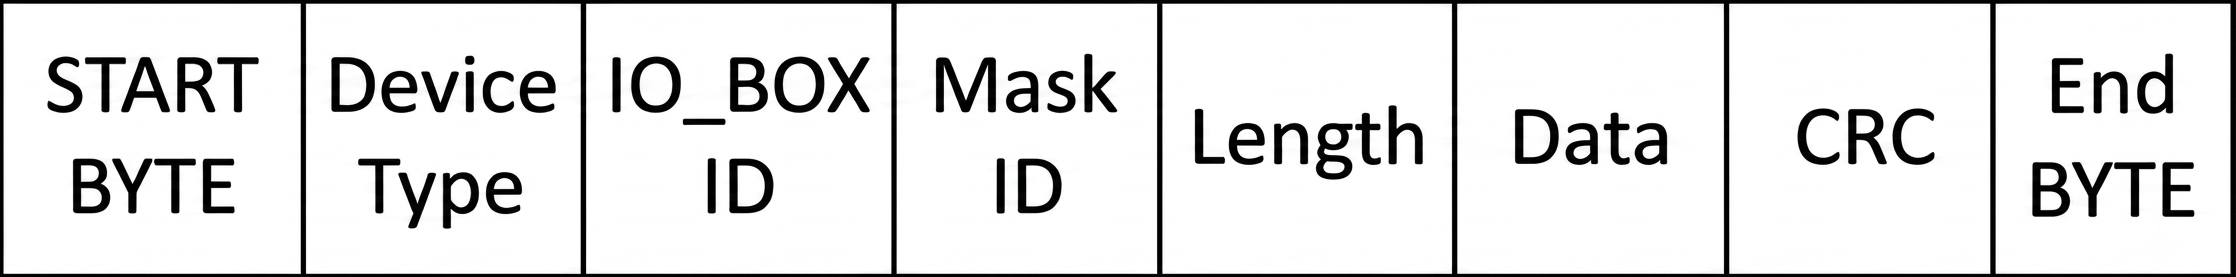
\includegraphics[width=\textwidth]{Figures/ioframe_structure.png}
    \caption{Structure of the IOBOX output frame}
    \label{fig:ioframe_structure}
\end{figure}

The frame assembly routine populates each field from the most recently 
persisted system state, then computes and appends a CRC checksum over all 
preceding fields. The complete frame format is described in detail below.

\paragraph{Start Byte.}
A fixed synchronisation marker (\texttt{0xAA}) that signals the beginning of a 
valid frame to any receiver scanning an incoming byte stream, allowing frame 
boundaries to be established without relying on inter-frame timing gaps.

\paragraph{Device Type.}
Identifies the category of the transmitting device, allowing a network to host 
multiple types of embedded nodes simultaneously. A receiving gateway inspects 
this field to apply the appropriate decoding logic without prior knowledge of 
the sender's identity.

\paragraph{IOBOX ID.}
Carries the unique numeric identifier of the specific IOBOX unit that generated 
the frame. In multi-node deployments, this field allows a receiving system to 
associate each frame with its physical origin without requiring any session or 
connection establishment.

\paragraph{Mask ID.}
A configuration bitmap describing which sensors and communication modules are 
active and contributing data to the current frame. Each bit corresponds to one 
module, as detailed in Table~\ref{tab:mask_id}. The receiver reads this field 
before parsing the payload to determine the exact byte layout of the Data field, 
providing both flexibility and forward compatibility.

\begin{table}[H]
    \centering
    \caption{Mask ID bit field definitions}
    \label{tab:mask_id}
    \begin{tabular}{|c|l|c|}
        \hline
        \textbf{Bit} & \textbf{Module} & \textbf{Logic 1 meaning} \\
        \hline
        5 & CAN sniffer             & CAN data present in payload \\
        \hline
        4 & HTS221TR Temperature    & HTS221 temperature present \\
        \hline
        3 & HTS221TR Humidity       & HTS221 humidity present \\
        \hline
        2 & ENS210 Temperature      & ENS210 temperature present \\
        \hline
        1 & ENS210 Humidity         & ENS210 humidity present \\
        \hline
        0 & OPT3001DNPR Illuminance & OPT3001 lux value present \\
        \hline
    \end{tabular}
\end{table}

\paragraph{Length.}
Specifies the total size of the Data field in bytes, making the frame 
self-describing. The receiver uses this field to locate the CRC and End Byte at 
their correct positions without re-deriving the payload size from the Mask ID.

\paragraph{Data.}
Contains the measurement values and communication data collected during the 
current acquisition cycle. Its contents are governed entirely by the active bits 
in the Mask ID field. In the current configuration, the payload includes 
temperature and humidity readings from both sensor units, the OPT3001DNPR 
illuminance value, and the CAN frame payload comprising the message identifier, 
RTR flag, data length code, and up to eight data bytes.

\paragraph{CRC.}
A 16-bit integrity checksum computed over all preceding fields using the 
CRC-16/IBM polynomial. The receiver verifies this field before consuming any 
measurement data; a mismatch indicates a transmission error or a corrupted frame 
and requires the frame to be discarded.

\paragraph{End Byte.}
A fixed termination marker (\texttt{0x55}) that constitutes a second layer of 
frame boundary validation. Together with the Start Byte, it allows the receiver 
to detect framing errors — for example, those caused by a corrupted Length field 
— even when the CRC alone might not reveal the misalignment.

The complete field layout is summarised in Table~\ref{tab:ioframe_fields}.

\begin{table}[H]
    \centering
    \caption{IoFrame field summary}
    \label{tab:ioframe_fields}
    \begin{tabular}{|l|l|p{6.5cm}|}
        \hline
        \textbf{Field} & \textbf{Value} & \textbf{Description} \\
        \hline
        Start Byte  & \texttt{0xAA}    & Frame synchronisation delimiter \\
        \hline
        Device Type & Compile-time constant & Node category identifier \\
        \hline
        IOBOX ID    & Compile-time constant & Per-unit unique identifier \\
        \hline
        Mask ID     & 6-bit bitmap     & Active module bitmap \\
        \hline
        Length      & Variable         & Data field length in bytes \\
        \hline
        Data        & Variable         & Active measurement payload \\
        \hline
        CRC         & CRC-16/IBM       & Integrity check over all preceding fields \\
        \hline
        End Byte    & \texttt{0x55}    & Frame termination delimiter \\
        \hline
    \end{tabular}
\end{table}

The frame assembly routine retrieves the last persisted system state and fills 
every field sequentially before computing and inserting the CRC. This design 
ensures that the output frame always reflects the most recently stored platform 
state, providing continuity across power cycles and making the frame contents 
auditable through the non-volatile storage layer.
\subsubsection{System Data Flow}

% --- Figure: data flow diagram ---
\begin{figure}[H]
    \centering
    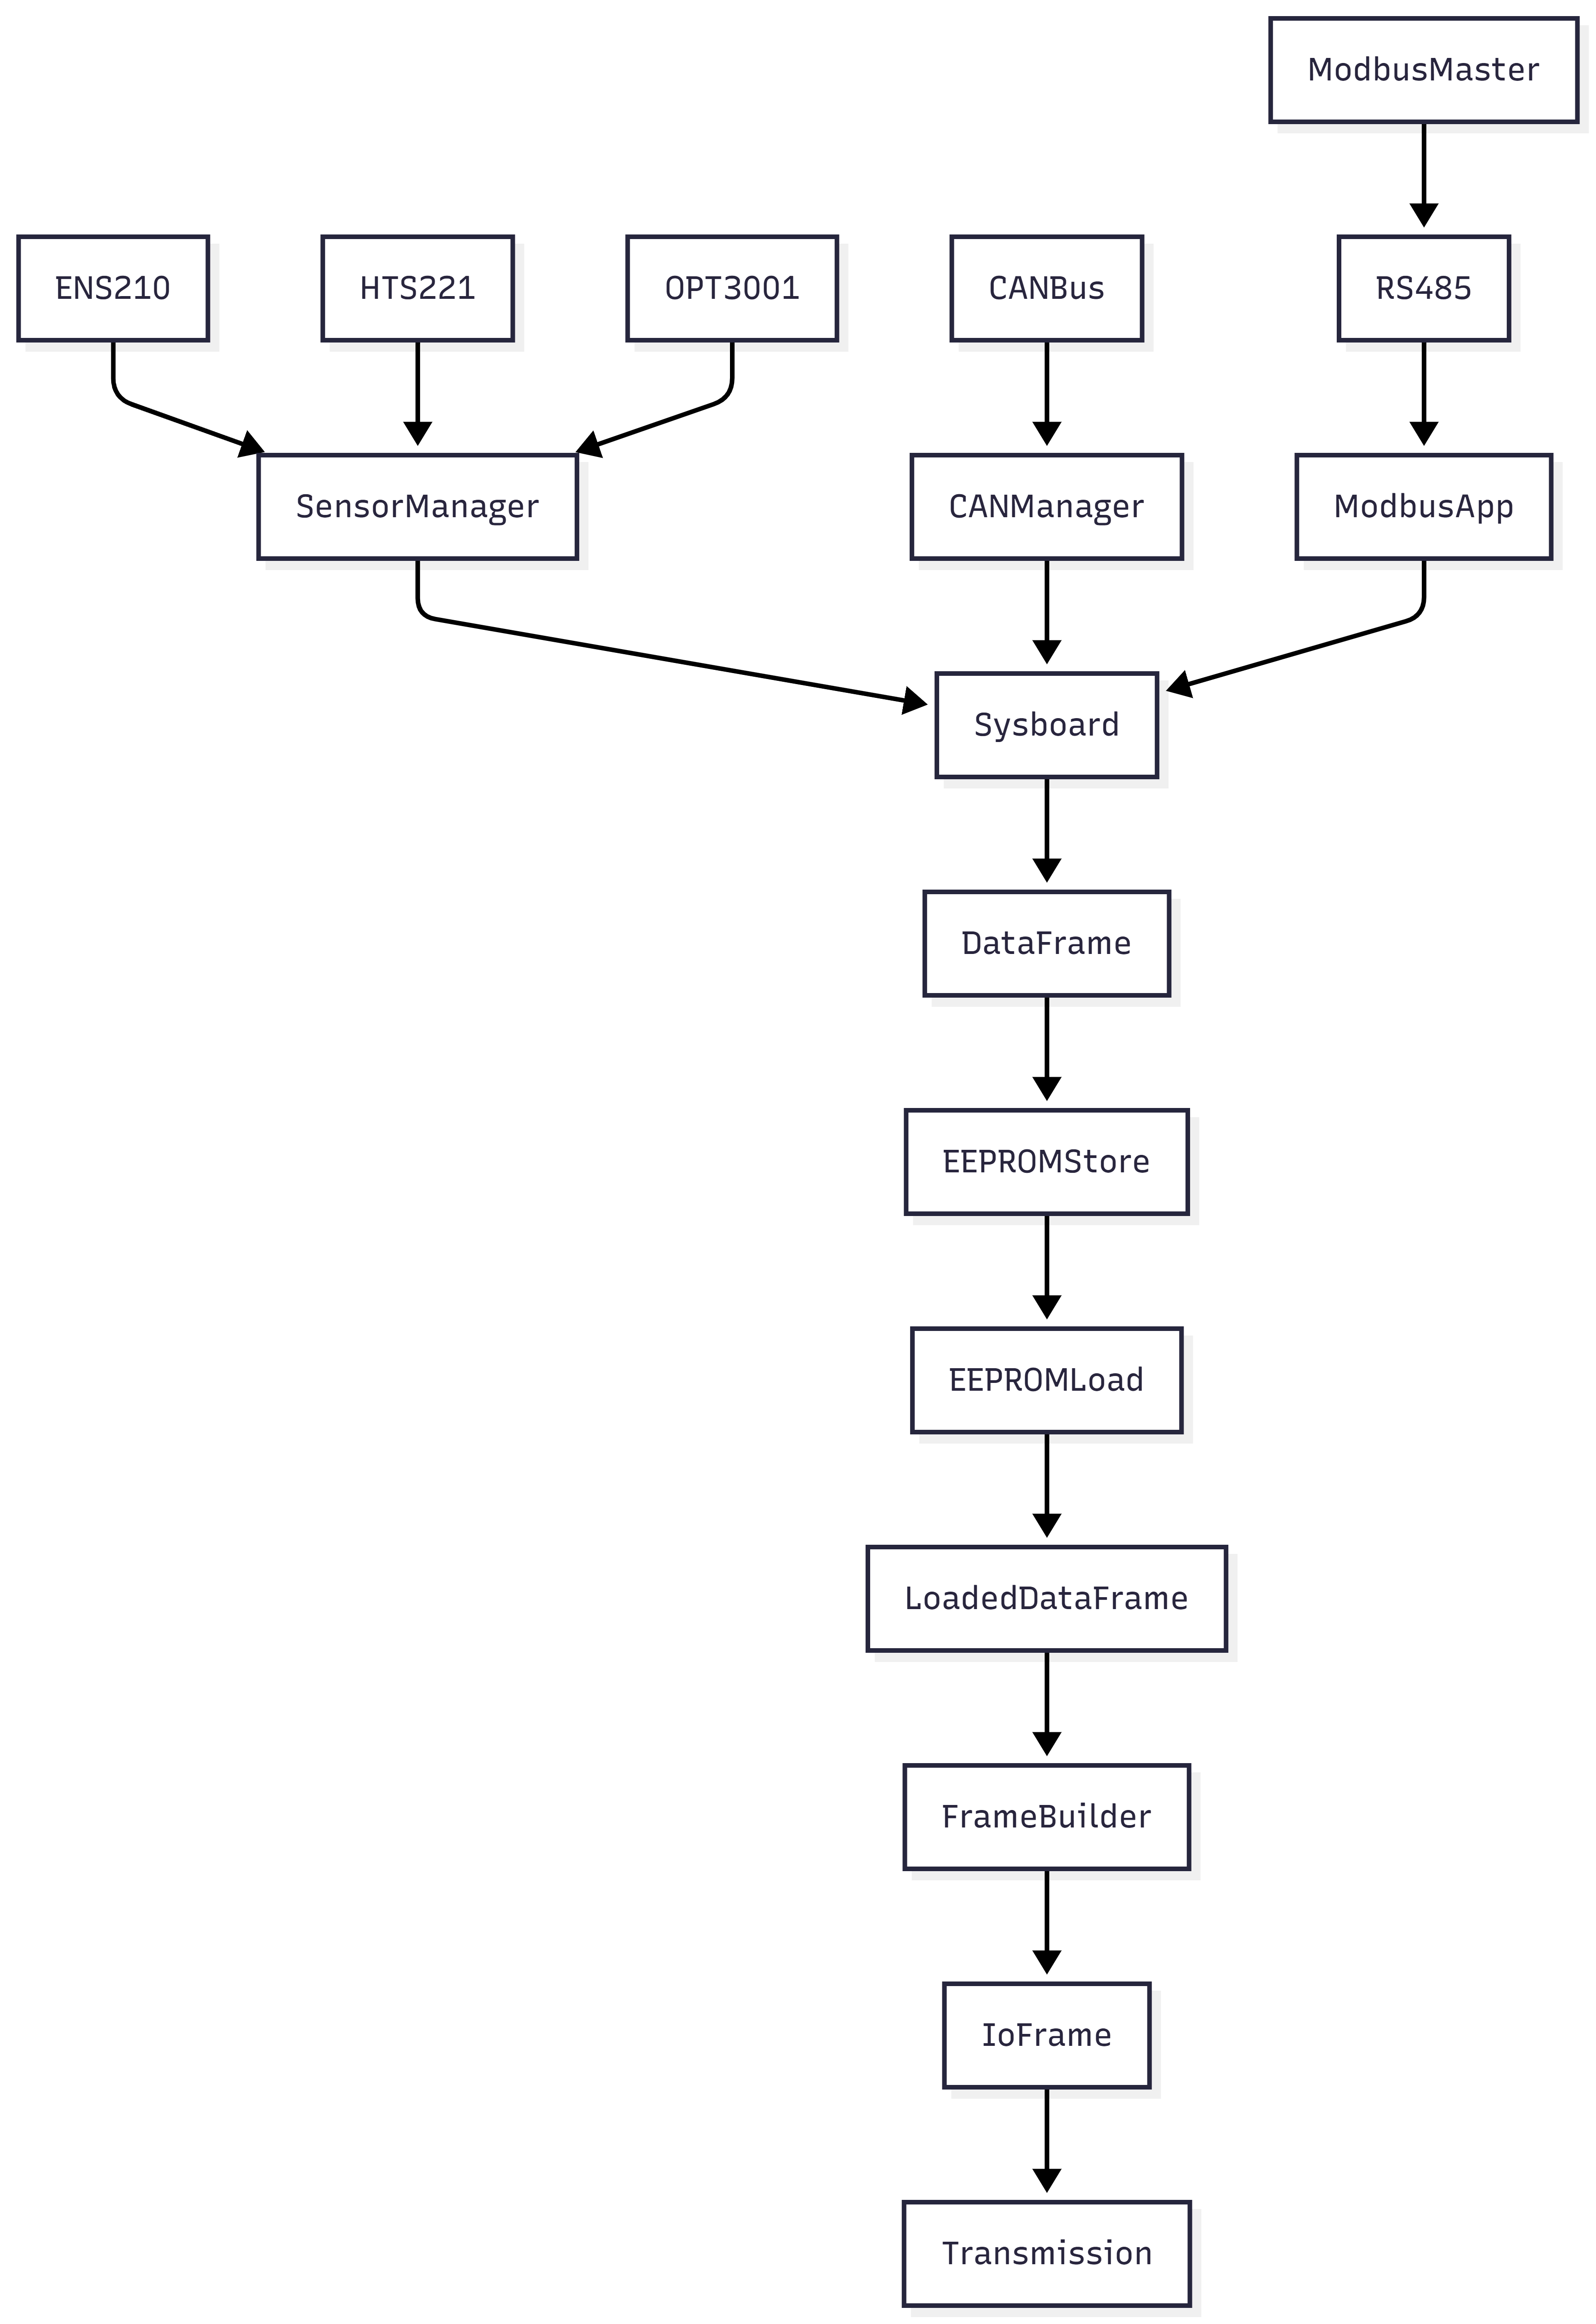
\includegraphics[width=0.85\textwidth]{Figures/data_flow.png}
    \caption{End-to-end data flow across the three firmware layers}
    \label{fig:data_flow}
\end{figure}

The complete data path through the system can be summarised as follows. Physical 
sensor measurements are acquired by the Sensor Module and written into 
\texttt{sysboard}. Simultaneously, CAN frames captured by the CAN Manager are 
stored in the same structure. At every 1000~ms interval, the EEPROM Store task 
serialises \texttt{sysboard} into a \texttt{DataFrame} and writes it to 
non-volatile memory; the EEPROM Load task immediately retrieves the last valid 
frame. Finally, the Frame Builder consumes the loaded \texttt{DataFrame} and 
produces the \texttt{IoFrame} output, ready for transmission. Throughout this 
pipeline, any Modbus master connected via RS485 may read live sensor values 
directly from \texttt{sysboard} through the Modbus Application Module at any 
point in the cycle.

\section*{} % transition placeholder — Conclusion follows
The software architecture described in this section provides a clean separation 
of concerns, compile-time configurability, and a deterministic execution model 
without the overhead of a real-time operating system. The following section 
presents the validation results obtained on the target hardware.

\section{Conclusion}

\bibliographystyle{plain}
\bibliography{References}
\end{document}

\cleardoublepage
\clearpage